\hypertarget{khung-sux1b0ux1eddn}{%
  \section{Khung sườn}\label{khung-sux1b0ux1eddn}}

Khung sườn khóa luận kết thúc 6 năm luyện ngục của nvmnghia.

Độ dài yêu cầu: 40-50 trang.

\begin{center}\rule{0.5\linewidth}{0.5pt}\end{center}

\hypertarget{buxeca-cuxe1c-mux1ee5c-liuxean-quan}{%
  \subsection{0. Bìa \& các mục liên
    quan}\label{buxeca-cuxe1c-mux1ee5c-liuxean-quan}}

\begin{itemize}
  \item
        Bìa
  \item
        Phụ bìa
  \item
        Cam đoan không sao chép
  \item
        Phê chuẩn của giảng viên hướng dẫn
  \item
        Lời cảm ơn
  \item
        Tóm tắt

        Nhờ Internet, truyền hình và điện ảnh, văn hóa truyện tranh đã trở nên
        phổ biến toàn cầu, nhất là trong giới trẻ. Nhu cầu tiêu thụ truyện
        tranh tăng cao thúc đẩy sự phát triển của các trang web truyện tranh
        với ưu điểm là thuận tiện, tốc độ cập nhật truyện nhanh. Tuy nhiên,
        nguồn truyện tranh của những trang web này có chất lượng không cao.
        Một bộ phận người đọc kĩ tính chọn đọc và lưu trữ những tệp truyện
        được số hóa chất lượng cao, thường ở dạng tệp nén đuôi \texttt{cbr} và
        \texttt{cbz}. Xuất phát từ nhu cầu này, tôi muốn viết ứng dụng
        \emph{yacv} có thể đọc các tệp truyện nén trên điện thoại Android.
        Khóa luận sẽ trình bày một số nền tảng của yacv như Android và Kotlin;
        sau đó là các ca sử dụng chính cùng với thiết kế và cài đặt của ứng
        dụng.

        Từ khóa: Android, coroutine, zip, comic
  \item
        Mục lục
  \item
        Danh sách bảng
  \item
        Danh sách hình
  \item
        Danh sách kí hiệu, chữ viết tắt

        \begin{itemize}
          
          \item
                MVC
          \item
                MVP
          \item
                MVVM
          \item
                AOT
          \item
                JIT
          \item
                API
          \item
                JS
          \item
                ES6
          \item
                RDBMS
          \item
                ACID
          \item
                ORM
          \item
                SC
        \end{itemize}
\end{itemize}

\begin{center}\rule{0.5\linewidth}{0.5pt}\end{center}

\hypertarget{chux1b0ux1a1ng-1-giux1edbi-thiux1ec7u}{%
  \subsection{\texorpdfstring{1. Chương 1: Giới thiệu
    }{1. Chương 1: Giới thiệu }}\label{chux1b0ux1a1ng-1-giux1edbi-thiux1ec7u}}

\hypertarget{ux111ux1eb7t-vux1ea5n-ux111ux1ec1}{%
  \subsubsection{\texorpdfstring{1.1. Đặt vấn đề
    }{1.1. Đặt vấn đề }}\label{ux111ux1eb7t-vux1ea5n-ux111ux1ec1}}

Tại Đông Á và Đông Nam Á, văn hóa truyện tranh gốc Á, nhất là truyện
tranh Nhật (manga), được đón nhận khá tích cực, đặc biệt trong giới trẻ.
Thế hệ những người dưới 40 tuổi hiện nay được tiếp xúc với truyện tranh
từ sớm, thông qua những cuốn truyện truyền tay và phim hoạt hình dựa
trên truyện tranh, và tiếp tục đọc dù đã qua tuổi thiếu niên. Một số tác
phẩm manga còn có lượng người đọc lớn trên toàn cầu như Doraemon, One
Piece. Ở bên kia bán cầu, với sự thành công của vũ trụ điện ảnh Marvel
và DC, truyện tranh phương Tây (comic) cũng được hồi sinh phần nào sau
một thập kỷ thiếu sáng tạo và suy giảm doanh số sách in. Các bộ truyện
siêu anh hùng, vốn trước đây chỉ phổ biến ở Hoa Kỳ, nay đang trên đường
trở thành một phần của văn hóa đại chúng như vị thế của manga. Có thể
nói, văn hóa truyện tranh nói chung đang ở thời kì phát triển mạnh, xét
theo tiêu chí về độ phổ biến và thái độ đón nhận của xã hội.

Hiện nay, hầu hết mọi người đọc truyện qua các trang web tổng hợp truyện
tranh. Những trang web này có hai ưu điểm chính:

\begin{itemize}
  
  \item
        Số lượng: Mỗi trang cung cấp ít nhất hàng nghìn đầu truyện.
  \item
        Tốc độ: Tốc độ ra truyện rất nhanh. Với các bộ truyện nổi tiếng,
        thường chỉ trong vòng một vài giờ sau khi ra mắt, chương mới đã xuất
        hiện.
\end{itemize}

Tuy vậy, nhược điểm chính của những trang web này là chất lượng ảnh của
truyện. Để giảm thời gian tải và tránh tốn băng thông, hình ảnh của
truyện thường được nén khá nhiều, gây vỡ hình, mờ nhòe. Một bộ phận
người đọc, hoặc kĩ tính, hoặc muốn sưu tầm truyện, thường chọn đọc những
tệp truyện chất lượng cao, thường có đuôi \texttt{.cbz} hoặc
\texttt{.cbr}. Bản chất tệp truyện này là các tệp nén zip bình thường,
bên trong có các tệp ảnh thông dụng như \texttt{.jpg}, \texttt{.png}.
Tuy nhiên, do được tải hẳn về máy rồi mới đọc, những tệp truyện này
không bị giới hạn về băng thông hay thời gian, do đó hình ảnh trong tệp
có thể có chất lượng rất cao.

Trong khóa luận này, tôi viết một ứng dụng Android nhằm phục vụ số ít
người dùng có nhu cầu đọc truyện tranh chất lượng cao đã giới thiệu ở
trên. Tên của ứng dụng là ``yacv'', viết tắt của cụm từ tiếng Anh ``Yet
Another Comic Viewer'', tạm dịch là ``Lại một ứng dụng xem truyện tranh
nữa''. Hai tính năng chính duy nhất của ứng dụng là đọc và quản lí cơ
bản (tìm kiếm, xóa) tệp truyện tranh có sẵn trên điện thoại.

Cần chú ý rằng ứng dụng yacv chỉ bao gồm các tính năng liên quan đến đọc
truyện ngoại tuyến, đọc các tệp truyện có sẵn trên điện thoại người
dùng. Ứng dụng không phải là ứng dụng khách cho các trang đọc truyện
hiện có, hay có máy chủ tập trung riêng để cung cấp truyện.

\hypertarget{ux1ee9ng-dux1ee5ng-tux1b0ux1a1ng-tux1ef1}{%
  \subsubsection{\texorpdfstring{1.2. Ứng dụng tương tự
    }{1.2. Ứng dụng tương tự }}\label{ux1ee9ng-dux1ee5ng-tux1b0ux1a1ng-tux1ef1}}

Hiện có nhiều ứng dụng đọc truyện tranh ngoại tuyến như yacv trên chợ
ứng dụng Google Play. Hai ứng dụng phổ biến nhất trong số này là
\href{https://play.google.com/store/apps/details?id=com.viewer.comicscreen\&hl=en\&gl=US}{ComicScreen}
và
\href{https://play.google.com/store/apps/details?id=com.aerilys.acr.android\&hl=en\&gl=US}{Astonishing
  Comic Reader}. ComicScreen là ứng dụng có nhiều người dùng hơn. Các tính
năng của ComicScreen giống với các tính năng của yacv, tuy nhiên
ComicScreen có thêm nhiều chức năng phụ, đáng kể nhất là khả năng đọc từ
mạng FTP/SMB và khả năng sửa ảnh trong file. Astonishing Comic Reader
cũng có chức năng tương tự yacv, không hơn, tuy nhiên giao diện khá trau
chuốt. Cả hai đều miễn phí và có quảng cáo, được cập nhật có thể nói là
thường xuyên.

Một ngoại lệ đáng kể ở đây là ứng dụng mã nguồn mở
\href{https://github.com/tachiyomiorg/tachiyomi}{Tachiyomi}. Ứng dụng
này có hệ thống phần mở rộng, cho phép đọc truyện ở các trang web truyện
tranh. Khi web truyện tranh thay đổi, hoặc hỗ trợ thêm trang mới, chỉ
cần tải về phần mở rộng tương ứng ở dạng ứng dụng \texttt{.APK}. Tính
năng này cùng mô hình mã nguồn mở khiến Tachiyomi mạnh hơn, cập nhật
nhanh hơn toàn bộ các ứng dụng đã có và sẽ có. Tuy nhiên, Tachiyomi lại
không thể được đưa lên Play Store, vì chính tính năng phần mở rộng đã
\href{https://github.com/tachiyomiorg/tachiyomi/issues/1745}{vi phạm
  chính sách} của Play Store.

Một điểm khác biệt quan trọng của yacv với các ứng dụng có sẵn là việc
hỗ trợ metadata của tệp truyện tranh, do các ứng dụng có sẵn trên Play
Store đa số bỏ qua thông tin này trong tệp truyện. Một trong số rất ít
những ứng dụng hỗ trợ tính năng này là
\href{https://play.google.com/store/apps/details?id=br.com.kurotoshiro.leitor_manga\&hl=en\&gl=US}{Kuro
  Reader}, tuy nhiên đây là một tính năng trả phí.

\hypertarget{kux1ebft-quux1ea3-ux111ux1ea1t-ux111ux1b0ux1ee3c}{%
  \subsubsection{\texorpdfstring{1.3. Kết quả đạt được
    }{1.3. Kết quả đạt được }}\label{kux1ebft-quux1ea3-ux111ux1ea1t-ux111ux1b0ux1ee3c}}

Ứng dụng có các tính năng đủ dùng theo mục đích đã đề ra:

\begin{itemize}
  
  \item
        Đọc file truyện \texttt{.cbz}
  \item
        Tìm kiếm truyện theo metadata
\end{itemize}

Tính năng đọc tệp truyện \texttt{.cbr} hiện mới chỉ được cài đặt một
phần, do khó khăn trong việc tích hợp thư viện đọc định dạng này.

\hypertarget{cux1ea5u-truxfac-khuxf3a-luux1eadn}{%
  \subsubsection{\texorpdfstring{1.4. Cấu trúc khóa luận
    }{1.4. Cấu trúc khóa luận }}\label{cux1ea5u-truxfac-khuxf3a-luux1eadn}}

Các phần còn lại của khóa luận có cấu trúc như sau:

\begin{itemize}
  
  \item
        \protect\hyperlink{P2-fundamental}{Chương 2 - Kiến thức nền tảng}:
        Giới thiệu sơ lược về ba nền tảng của ứng dụng, gồm hệ điều hành
        Android, ngôn ngữ lập trình Kotlin, và mẫu thiết kế MVVM; định dạng
        tệp nén \texttt{.zip} cũng được giới thiệu vì liên quan trực tiếp đến
        ứng dụng.
  \item
        \protect\hyperlink{P3-specification}{Chương 3 - Phân tích yêu cầu}:
        Phân tích nhu cầu và ca sử dụng để có đặc tả yêu cầu.
  \item
        \protect\hyperlink{P4-design}{Chương 4 - Thiết kế}: Thiết kế ứng dụng,
        gồm thiết kế cơ sở dữ liệu, giao diện, logic nghiệp vụ.
  \item
        \protect\hyperlink{P5-implementation}{Chương 5 - Lập trình \& Kiểm
          thử}: Một số cài đặt và ca kiểm thử trong ứng dụng sẽ được nêu một
        cách có chọn lọc.
  \item
        \protect\hyperlink{P6-comclusion}{Chương 6 - Kết luận}: Kết thúc khóa
        luận.
\end{itemize}

\begin{center}\rule{0.5\linewidth}{0.5pt}\end{center}

\hypertarget{chux1b0ux1a1ng-2-kiux1ebfn-thux1ee9c-nux1ec1n-tux1ea3ng}{%
  \subsection{\texorpdfstring{2. Chương 2: Kiến thức nền tảng
    }{2. Chương 2: Kiến thức nền tảng }}\label{chux1b0ux1a1ng-2-kiux1ebfn-thux1ee9c-nux1ec1n-tux1ea3ng}}

Chương này giới thiệu sơ qua về các nền tảng trong quá trình xây dựng
ứng dụng.

\begin{itemize}
  
  \item
        Hai nền tảng đầu tiên liên quan đến nhau, là tiền đề cho toàn bộ ứng
        dụng sẽ được giới thiệu trước, gồm hệ điều hành Android và ngôn ngữ
        lập trình Kotlin.
  \item
        Tiếp theo, lựa chọn về kiến trúc tổng quan, liên quan đến giao diện
        của ứng dụng được trình bày.
  \item
        Sau đó, cơ sở dữ liệu một số phần mở rộng của nó dùng trong ứng dụng
        sẽ được nhắc qua.
  \item
        Cuối cùng là thông tin về \texttt{.cbz} - định dạng tệp tin mà ứng
        dụng đọc, gồm hai phần: sơ lược về định dạng \texttt{.zip} mà
        \texttt{.cbz} dựa trên, và các trường metadata trong tệp tin
        \texttt{.cbz} - nguồn thông tin quan trọng để quản lí truyện.
\end{itemize}

\hypertarget{hux1ec7-ux111iux1ec1u-huxe0nh-android}{%
  \subsubsection{\texorpdfstring{2.1. Hệ điều hành Android
    }{2.1. Hệ điều hành Android }}\label{hux1ec7-ux111iux1ec1u-huxe0nh-android}}

Android là một hệ điều hành do Google phát triển cho thiết bị di động.
Android dùng nhân Linux và được thiết kế cho màn hình cảm ứng. Cùng với
iOS của Apple, Android trở thành một phần không thể thiếu của cuộc cách
mạng di động bắt đầu vào cuối những năm 2000.

Google mua lại phiên bản Android đầu của công ty khởi nghiệp cùng tên
vào năm 2005, và phát triển hệ điều hành này từ đó. Ngoài Google,
Android còn nhận đóng góp lớn từ cộng đồng, do là một dự án mã nguồn mở
(phần lớn mã nguồn dùng giấy phép Apache); tên chính thức của dự án là
Android Open Source Project. Dù vậy, mọi thiết bị Android thương mại đều
có ứng dụng độc quyền. Ví dụ đáng kể là bộ Google Mobile Service, chứa
những ứng dụng không thể thiếu như trình duyệt Chrome hay chợ Play
Store. Về mặt này, Android khá giống Chrome: thành phần cốt lõi kĩ thuật
được phát triển theo mô hình mã nguồn mở (AOSP và Chromium), còn thành
phần liên quan đến trải nghiệm người dùng được phát triển riêng.

\begin{figure}
  \centering
  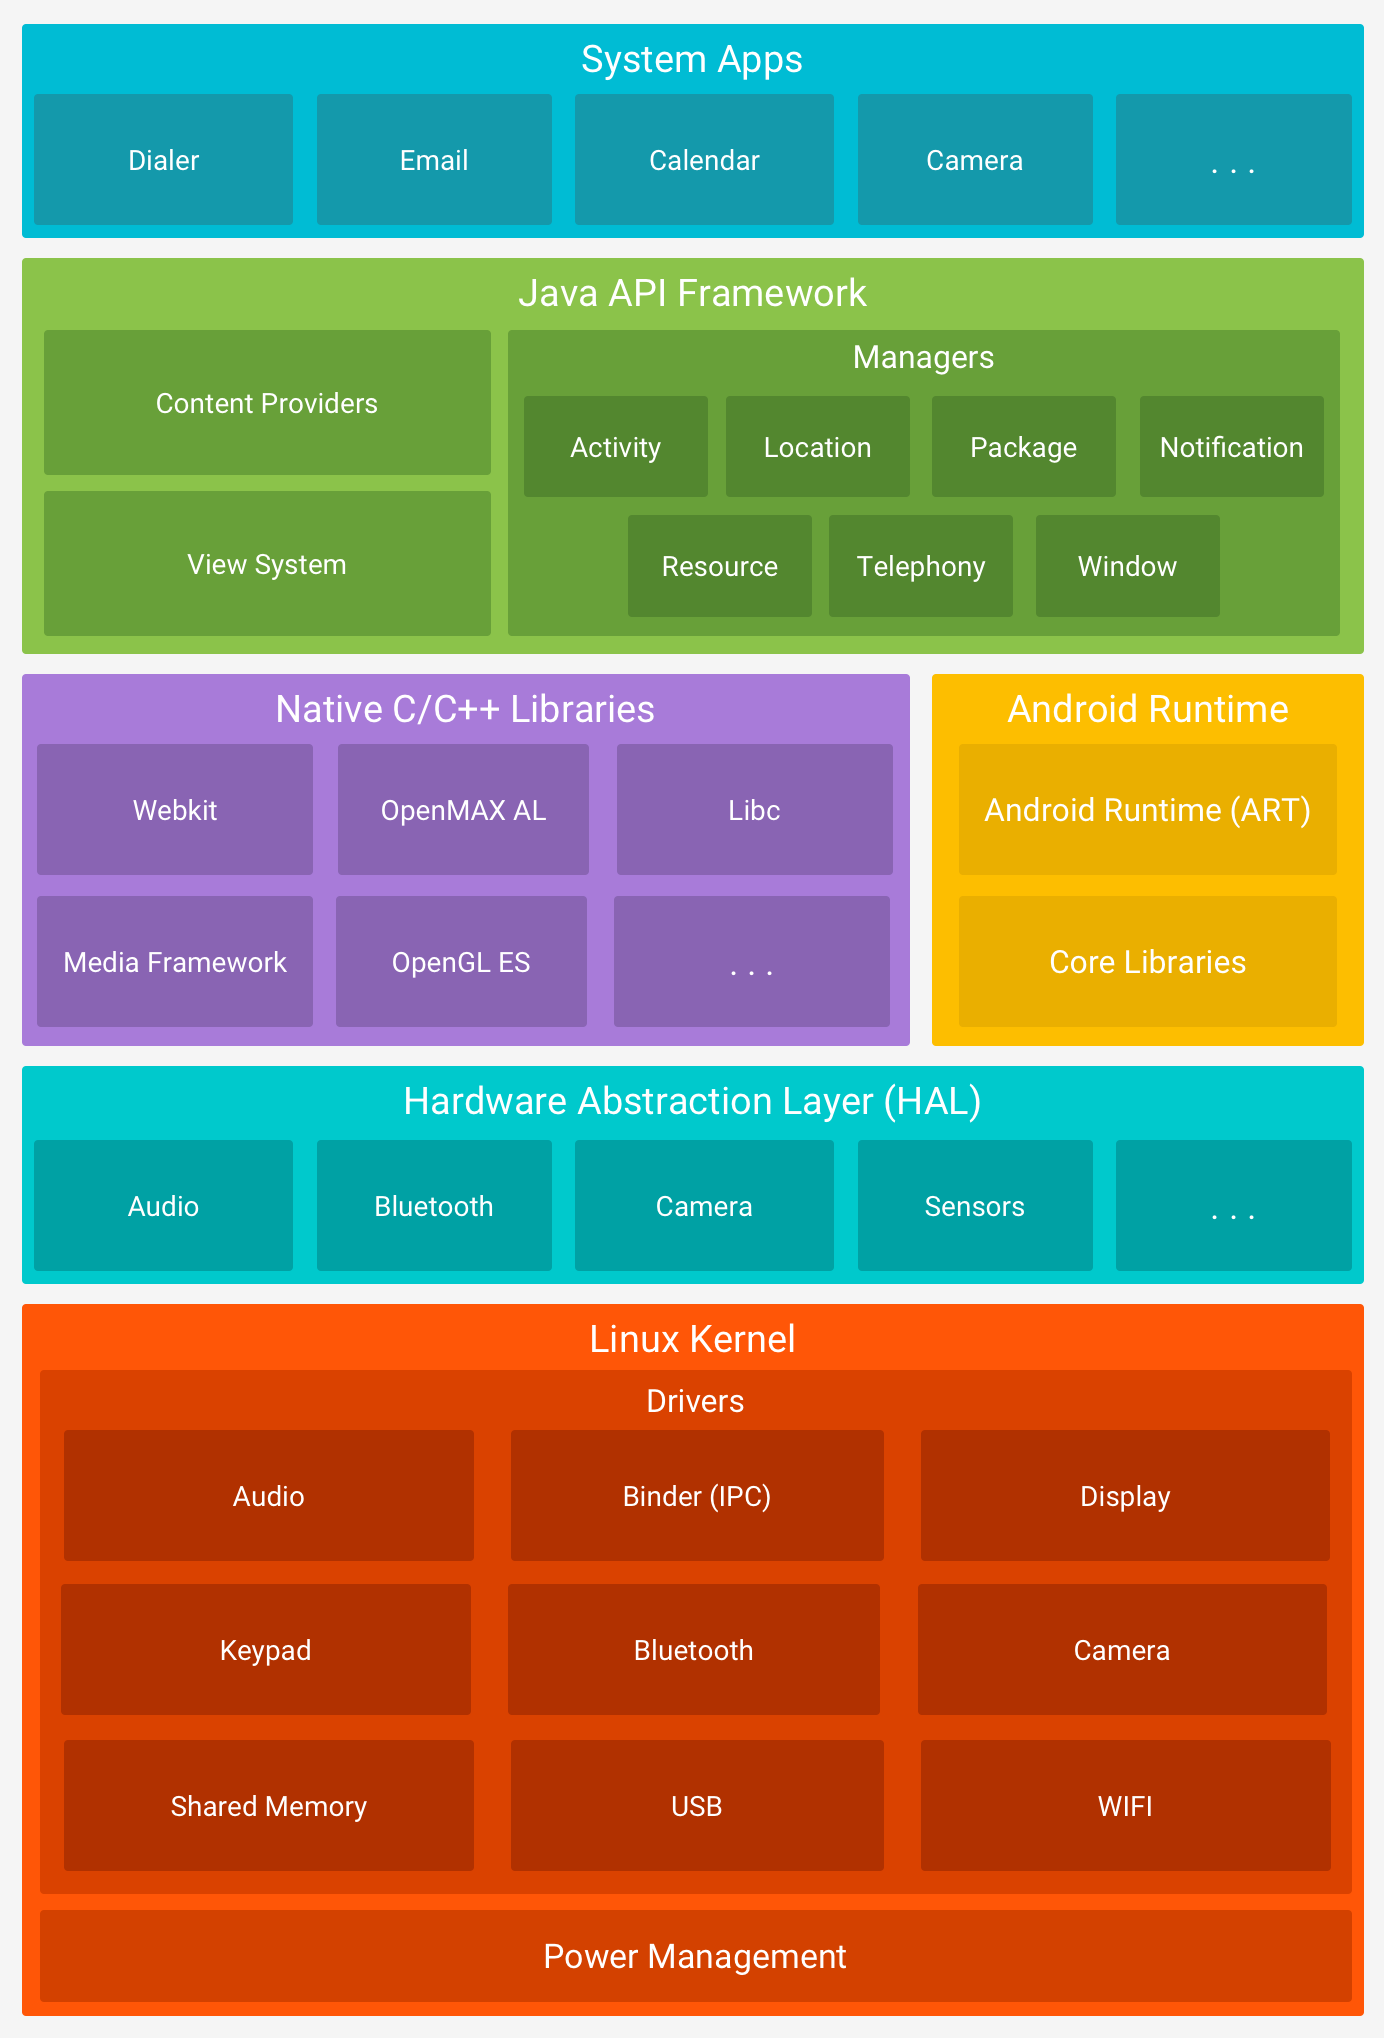
\includegraphics{../images/android-stack_2x.png}
  \caption{Android software stack}
\end{figure}

Hình 1. Các phân lớp của hệ điều hành Android

Hệ điều hành Android được phân lớp như sau:

\begin{itemize}
  \item
        Nhân Linux (Linux Kernel):

        Đây là tầng thấp nhất. Android dùng nhánh hỗ trợ dài hạn (LTS) của
        Linux. Không như kiểu phát triển distro trên máy tính (chủ yếu thay
        đổi ở ngoài nhân), Google sửa và thêm bớt nhiều thành phần vào nhân
        trước khi tích hợp.
  \item
        Lớp phần cứng trừu tượng (Hardware Abstraction Layer):

        Tầng này trừu tượng hóa các chi tiết phần cứng bằng cách đưa ra các
        giao diện chung cho một kiểu phần cứng nào đó, giúp các tầng trên
        không cần quan tâm đến chi tiết riêng của phần cứng.
  \item
        Android Runtime (ART):

        Ứng dụng Java cần thêm một ứng dụng để chuyển bytecode thành mã máy.
        Trên desktop, đó là các máy ảo Java (JVM). Trên Android, Android
        Runtime nhận nhiệm vụ này. Hai máy ảo này khác nhau ở chỗ ART
        \emph{biên dịch} bytecode thành mã máy (trước khi chạy - AOT), còn JVM
        \emph{thông dịch} bytecode thành mã máy (trong khi chạy).

        ART hiện hỗ trợ đa số tính năng của Java 8.
  \item
        Thư viện C/C++:

        Tầng thư viện native nằm ngang hàng với ART, phục vụ các tiến trình hệ
        thống và một số ứng dụng dùng NDK (tức gọi API C cấp thấp) như trò
        chơi điện tử.
  \item
        Khung phát triển ứng dụng (Java API Framework):

        Mọi ứng dụng Java được viết nhờ sử dụng các thành phần của tầng này
        thông qua API Java. Tầng này cung cấp toàn bộ tính năng của Android
        cho lập trình viên, bao gồm các yếu tố cơ bản như giao diện (View
        System), truy xuất,\ldots{}

        Lập trình viên có quyền truy cập vào lớp này tương đương với ứng dụng
        hệ thống. Đây có thể coi là một cam kết tránh độc quyền công nghệ, tức
        đa số ứng dụng hệ thống không có khả năng đặc biệt, hay hiệu năng cao
        hơn ứng dụng bên thứ ba tương tự.
  \item
        Ứng dụng hệ thống (System Apps)

        Android đi kèm với một số ứng dụng hệ thống như ứng dụng SMS, trình
        duyệt, lịch,\ldots{} Google cho phép thay thế đa số các ứng dụng này
        với ứng dụng bên thứ ba, tuy nhiên có những ngoại lệ như ứng dụng Cài
        đặt (Settings).
\end{itemize}

Gần như mọi ứng dụng Android cơ bản đều sử dụng thành phần View System
trong tầng Khung phát triển để viết giao diện, và yacv không là ngoại
lệ. yacv còn sử dụng thành phần Content Provider, cụ thể là bộ Storage
Access Framework, và sẽ được đề cập ở các phần sau.

\hypertarget{android-jetpack}{%
  \paragraph{\texorpdfstring{2.1.1. Android Jetpack
    }{2.1.1. Android Jetpack }}\label{android-jetpack}}

Jetpack là bộ thư viện giúp viết ứng dụng Android nhanh gọn, ít lỗi hơn
so với việc tự viết những đoạn mã tương tự. Jetpack gồm hai thành phần:

\begin{itemize}
  
  \item
        AndroidX: đưa API của phiên bản hệ điều hành mới lên máy cũ
  \item
        Architecture Component: đưa ra API hoàn toàn mới để giải quyết một vấn
        đề
\end{itemize}

Việc Google cho phép nhà sản xuất tùy biến khiến thế giới Android bị phân mảnh,
hệ quả là việc cập nhật hệ điều hành khó khăn. Do đó, Google viết Thư viện Hỗ
trợ (Support Library) để đưa API hệ điều hành mới lên máy cũ. AndroidX chính là
Support Library đổi tên và được cập nhật đến nay.

Chú ý rằng Jetpack chỉ có ích cho lập trình viên (được dùng API mới tiện
hơn, thực ra là wrapper của API sẵn có), chứ không cập nhật tính năng hệ
điều hành.

yacv sử dụng nhiều thành phần của Jetpack, trong đó đáng kể đến ba thư
viện sau:

\begin{itemize}
  
  \item
        LiveData: giúp giao diện luôn được cập nhật theo dữ liệu mới nhất
  \item
        ViewModel: giúp tách dữ liệu và giao diện
  \item
        Room: giúp việc lưu dữ liệu trong SQLite thuận tiện hơn
\end{itemize}

Room là một phần quan trọng của yacv, do đó sẽ được giới thiệu chi tiết
hơn ở \protect\hyperlink{P2.4.2-room}{mục sau}.

\hypertarget{nguxf4n-ngux1eef-lux1eadp-truxecnh-kotlin}{%
  \subsubsection{\texorpdfstring{2.2. Ngôn ngữ lập trình Kotlin
    }{2.2. Ngôn ngữ lập trình Kotlin }}\label{nguxf4n-ngux1eef-lux1eadp-truxecnh-kotlin}}

Java là ngôn ngữ lập trình đầu tiên được hỗ trợ trên Android, nhưng
không phải duy nhất. Từ 2019, Google khuyên lập trình viên viết ứng dụng
trên Kotlin, một ngôn ngữ mới do JetBrains phát triển. Giới thiệu lần
đầu vào năm 2011, Kotlin được định hướng trở thành lựa chọn thay thế cho
Java. Điều đó thể hiện ở việc Kotlin tương thích hoàn toàn với Java (từ
Java gọi được Kotlin và ngược lại), do cùng được biên dịch thành JVM
bytecode.

Điểm mạnh của Kotlin so với Java là tính ngắn gọn. Do được phát triển
mới, Kotlin không cần tương thích với phiên bản cũ, cho phép dùng các cú
pháp hiện đại, gọn ghẽ. Ngoài ra, vì được một công ty tư nhân phát
triển, Kotlin không cần chờ đến các cuộc họp phức tạp để đạt đồng thuận
về tính năng mới, giúp ngôn ngữ liên tục được cải tiến. Đồng thời, công
ty cũng mở mã nguồn của Kotlin và chương trình dịch, giúp đẩy nhanh quá
trình phát triển và tạo thiện cảm cộng đồng cho một ngôn ngữ non trẻ.

Sau đây là tóm tắt một số đặc điểm kĩ thuật của Kotlin:

\begin{itemize}
  
  \item
        Về mô hình, Kotlin hỗ trợ hướng đối tượng như Java, nhưng còn có hướng
        hàm, thể hiện ở tính năng hàm ẩn danh (lambda), và hàm được coi là
        first-class.
  \item
        Về hệ thống kiểu, Kotlin giống hệt Java:

        \begin{itemize}
          
          \item
                Là kiểu tĩnh (statically typed), tức kiểu được kiểm tra khi biên
                dịch (thay vì khi chạy, như Python, JavaScript,\ldots)
          \item
                Là kiểu mạnh (strongly typed), tức không cho phép chuyển kiểu ngầm
        \end{itemize}
  \item
        Về cú pháp, Kotlin có cú pháp gọn, hiện đại, ví dụ như bỏ dấu
        \texttt{;} cuối dòng, template literal,\ldots{}
  \item
        Về lỗi, Kotlin luôn được quảng cáo về khả năng chống
        \texttt{NullPointerException}. Kotlin ``né'' lỗi này do buộc người
        viết đánh dấu cụ thể rằng một đối tượng có thể bị \texttt{null} hay
        không bằng hậu tố \texttt{?} ở khai báo kiểu. Từ đó, Kotlin biết chính
        xác đối tượng có thể là \texttt{null} hay không, và buộc xử lí nếu có.
\end{itemize}

Do Google khuyên dùng Kotlin khi viết ứng dụng Android, tôi cho rằng
khóa luận này là một cơ hội phù hợp để thử Kotlin thay vì dùng Java quen
thuộc, và quyết định chọn viết yacv bằng Kotlin.

\hypertarget{coroutine}{%
  \paragraph{\texorpdfstring{2.2.1. Coroutine
    }{2.2.1. Coroutine }}\label{coroutine}}

\hypertarget{giux1edbi-thiux1ec7u-chung}{%
  \subparagraph{2.2.1.1. Giới thiệu
    chung}\label{giux1edbi-thiux1ec7u-chung}}

Một thư viện quan trọng của kotlin là \emph{coroutine}. Coroutine giúp
viết ứng dụng có tính tương tranh (concurrency) và bất đồng bộ
(asynchronous) một cách đơn giản hơn.

Về cơ bản, coroutine giống với luồng (thread), nhưng nhẹ hơn. Coroutine
luôn dùng mô hình \emph{đa nhiệm hợp tác} (cooperative multitasking),
khác với luồng hay dùng đa nhiệm ưu tiên (preemptive multitasking). Mấu
chốt khác biệt của chúng là đa nhiệm hợp tác có các ``điểm dừng'' do
người viết tạo; khi chạy đến đó, coroutine có thể dừng lại, chủ động nhả
CPU cho việc khác, rồi tiếp tục việc đang dở vào lúc thích hợp. Ngược
lại, đa nhiệm ưu tiên có thể buộc một luồng đang chạy ngừng lại bất kì
lúc nào để ưu tiên chạy một luồng khác. Đây cũng là điểm khiến coroutine
nhẹ hơn: chi phí chuyển ngữ cảnh (context switching) được kiểm soát và
cắt giảm, do chuyển sang thực thi một coroutine khác chưa chắc đã chuyển
sang một luồng hệ điều hành khác.

Với những điều trên, coroutine chưa làm được nhiều. Roman Elizarov,
trưởng dự án Kotlin, hướng coroutine trong Kotlin theo một ý tưởng mới:
\emph{tương tranh có cấu trúc} (structured concurrency, từ đây gọi tắt
là SC). Ý tưởng này tiếp tục đơn giản hóa việc viết những đoạn mã tương
tranh bằng cách áp đặt một số giới hạn, cấu trúc cơ bản. Kết quả là
coroutine trong Kotlin hỗ trợ việc xử lí lỗi và ngừng tác vụ bất đồng bộ
tốt hơn việc dùng luồng, hay các thư viện tương tranh như RxJava.

Coroutine được dùng để tăng tốc những đoạn mã chạy chậm trong yacv (sẽ
được mô tả sau). Ngoài cải thiện về hiệu năng, coroutine và tương tranh
có cấu trúc còn cho phép viết mã ngắn gọn, rõ ràng hơn. Do có tác động
lớn, coroutine sẽ được giới thiệu kĩ hơn ở phần này.

\hypertarget{buxe0i-hux1ecdc-tux1eeb-quuxe1-khux1ee9-lux1eadp-truxecnh-cuxf3-cux1ea5u-truxfac}{%
  \subparagraph{2.2.1.2. Bài học từ quá khứ: lập trình có cấu
    trúc}\label{buxe0i-hux1ecdc-tux1eeb-quuxe1-khux1ee9-lux1eadp-truxecnh-cuxf3-cux1ea5u-truxfac}}

Để hiểu về SC, ta có thể so sánh nó với \emph{lập trình có cấu trúc}
(structured programming). Để hiểu sơ về lập trình có cấu trúc, ta phải
tìm về \emph{lập trình phi cấu trúc} (non-structured programming), với
đặc điểm là lệnh nhảy \texttt{GOTO}. Trong buổi đầu của máy tính, lệnh
này được dùng nhiều vì hợp với cách máy tính chạy.

\begin{figure}
  \centering
  
\includegraphics{../images/sequential-and-go-to-schematic.svg}
  \caption{non-structured programming}
\end{figure}

Hình 2: Lập trình phi cấu trúc với \texttt{GOTO}

\begin{figure}
  \centering
  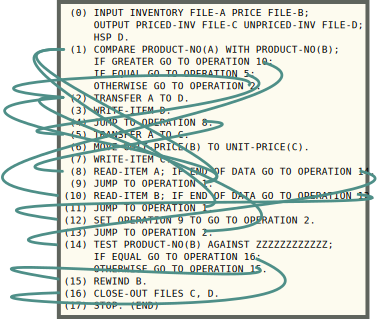
\includegraphics{../images/flow-matic-4.svg}
  \caption{spaghetti of goto}
\end{figure}

Hình 3: Sự lộn xộn của lập trình phi cấu trúc

Vấn đề của lập trình phi cấu trúc, hay của \texttt{GOTO}, có thể tóm gọn
như sau:

\begin{itemize}
  \item
        Khó nắm bắt luồng chương trình

        Khi đã chạy \texttt{GOTO}, các lệnh phía sau nó không biết khi nào mới
        chạy, vì chương trình chuyển sang lệnh khác mà không trở lại. Luồng
        chạy trở thành một đống ``mì trộn'' như Hình 3, thay vì tuần tự từ
        trên xuống. Tệ hơn, tính trừu tượng bị phá vỡ: khi gọi hàm, thay vì có
        thể bỏ qua chi tiết bên trong, ta phải biết rõ để xem có lệnh nhảy bất
        ngờ nào không.
  \item
        Không cài đặt được các chức năng mới (ngoại lệ, quản lí tài nguyên tự
        động,\ldots)

        Xét ví dụ Java sau về quản lí tài nguyên tự động:

        \begin{Shaded}
          \begin{Highlighting}[]
            \KeywordTok{try}\NormalTok{ (}\BuiltInTok{Scanner}\NormalTok{ scanner = }\KeywordTok{new} \BuiltInTok{Scanner}\NormalTok{(}\KeywordTok{new} \BuiltInTok{File}\NormalTok{(}\StringTok{"test.txt"}\NormalTok{))) \{}
            \FunctionTok{jumpSomewhere}\NormalTok{();    }\CommentTok{// Giả sử Java có GOTO, và hàm này dùng nó}
            \NormalTok{\}}
          \end{Highlighting}
        \end{Shaded}

        Do không trả lại luồng điều khiển, việc đóng luồng nhập từ tệp cũng
        không chắc chắn xảy ra, dẫn đến rò rỉ tài nguyên, làm khối lệnh vô
        dụng.

        Điều gần tương tự cũng khiến việc xử lí ngoại lệ và nhiều tính năng
        khác trở nên rất khó đạt được, một khi ngôn ngữ cho phép
        \texttt{GOTO}.
\end{itemize}

Lập trình có cấu trúc đơn giản hóa luồng chạy bằng cách giới hạn các
lệnh nhảy còn \texttt{if}, \texttt{for} và gọi hàm. Khác biệt mấu chốt
của ba lệnh này so với \texttt{GOTO} là chúng \emph{trả luồng điều
  khiển} về điểm gọi, thể hiện rõ ở Hình 4. Theo định nghĩa, ba lệnh trên
giải quyết được hậu quả đầu tiên. Đồng thời, các hậu quả số hai cũng
được giải quyết, do ngôn ngữ đã có cấu trúc (cụ thể là có call stack).

\begin{figure}
  \centering
  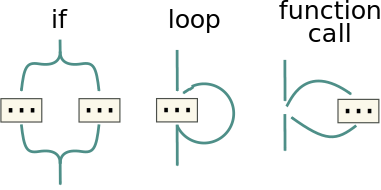
\includegraphics{../images/control-schematics.svg}
  \caption{3 basic constructs}
\end{figure}

Hình 4: Ba cấu trúc cơ bản của lập trình có cấu trúc: rẽ nhánh
\texttt{if}, lặp \texttt{for} và gọi hàm

Ngày nay, ba cấu trúc trên đã trở thành phần không thể thiếu trong mọi
ngôn ngữ lập trình, và \texttt{GOTO} chỉ còn dùng trong hợp ngữ. Quá khứ
cho thấy nếu áp dụng một số cấu trúc, giới hạn, ta có thể giải quyết vấn
đề một cách tinh tế và gọn gàng. Trong trường hợp này, SC có thể loại bỏ
một số điểm yếu của các API tương tranh/bất đồng bộ truyền thống, giống
cách lập trình có cấu trúc đã làm.

\hypertarget{uxe1p-dux1ee5ng-vuxe0o-hiux1ec7n-tux1ea1i-tux1b0ux1a1ng-tranh-cuxf3-cux1ea5u-truxfac}{%
  \subparagraph{2.2.1.3. Áp dụng vào hiện tại: tương tranh có cấu
    trúc}\label{uxe1p-dux1ee5ng-vuxe0o-hiux1ec7n-tux1ea1i-tux1b0ux1a1ng-tranh-cuxf3-cux1ea5u-truxfac}}

Trước hết, ta xem xét hai kiểu API tương tranh hay dùng hiện nay:

\begin{longtable}[]{@{}lll@{}}
  \toprule
  \begin{minipage}[b]{0.19\columnwidth}\raggedright
    Tên\strut
  \end{minipage} & \begin{minipage}[b]{0.46\columnwidth}\raggedright
    Giải thích\strut
  \end{minipage} & \begin{minipage}[b]{0.27\columnwidth}\raggedright
    Ví dụ\strut
  \end{minipage}\tabularnewline
  \midrule
  \endhead
  \begin{minipage}[t]{0.19\columnwidth}\raggedright
    Tương tranh\strut
  \end{minipage} & \begin{minipage}[t]{0.46\columnwidth}\raggedright
    Chạy một hàm theo cách tương tranh với luồng chạy hiện tại\strut
  \end{minipage} & \begin{minipage}[t]{0.27\columnwidth}\raggedright
    \texttt{Thread(target=fn).start()\ \#\ Python}\strut
  \end{minipage}\tabularnewline
  \begin{minipage}[t]{0.19\columnwidth}\raggedright
    Bất đồng bộ\strut
  \end{minipage} & \begin{minipage}[t]{0.46\columnwidth}\raggedright
    Chạy một hàm khi có sự kiện xảy ra (callback)\strut
  \end{minipage} & \begin{minipage}[t]{0.27\columnwidth}\raggedright
    \texttt{element.onclick\ =\ cb;\ //\ JS}\strut
  \end{minipage}\tabularnewline
  \bottomrule
\end{longtable}

Bảng 2: Hai kiểu API tương tranh thường thấy.

Qua Hình 5, không khó để thấy rằng mọi vấn đề của lập trình phi cấu trúc
đều lặp lại với hai API trên:

\begin{figure}
  \centering
  
\includegraphics{../images/sequential-and-go-to-schematic.svg}
  \caption{non-structured concurrency}
\end{figure}

Hình 5: Tương tranh phi cấu trúc với \texttt{goroutine} - API thuộc kiểu
tương tranh.

\begin{itemize}
  
  \item
        Ta xem lại ví dụ về quản lí tài nguyên tự động. Nếu có một luồng thực
        thi khác tương tranh với luồng chính, thì khi luồng chính đóng
        \texttt{Scanner}, có thể luồng kia vẫn đang đọc nó. Do đó, tính năng này
        không thể hoạt động.
  \item
        Với tính năng bắt ngoại lệ, nếu có ngoại lệ ở luồng tương tranh, ta
        cũng không có cách nào để biết, và buộc phải kệ nó.
\end{itemize}

Trên thực tế, có cách để thực hiện một số chức năng trên với API hiện
tại, tuy vậy đó đều là cách xử lí riêng, do đó chưa thực sự thuận tiện
khi dùng. Ví dụ, ES6 có \texttt{catch()} để bắt ngoại lệ trong
\texttt{Promise} mà không (thể) dùng cấu trúc \texttt{try-catch} sẵn có.
Với SC, các vấn đề này đều được giải quyết.

Ta xét một đoạn mã tương tranh dùng coroutine trong Kotlin, tức dùng SC
(không phải coroutine trong mọi ngôn ngữ đều dùng mô hình này):

\begin{figure}
  \centering
  \includegraphics{../images/kotlin-coroutine.svg}
  \caption{kotlin coroutine}
\end{figure}

Hình 6: Tương tranh có cấu trúc dùng coroutine trong Kotlin

Đoạn mã trong Hình 6 làm những việc sau:

\begin{itemize}
  \item
        Hàm \texttt{launch()} tạo ra các coroutine:

        \begin{itemize}
          
          \item
                \texttt{launch()} đầu tiên tạo ra coroutine \emph{cha}
          \item
                \texttt{launch()} thứ hai tạo ra coroutine \emph{con}, chạy hàm
                \texttt{A()}
          \item
                Tương tự, có một coroutine con chạy hàm \texttt{B()}
        \end{itemize}
  \item
        3 coroutine chạy ``song song'', chính xác hơn là tương tranh
\end{itemize}

Nguyên tắc của SC là: \emph{coroutine cha chờ mọi coroutine con chạy
  xong}, kể cả khi nó xong trước. Nguyên tắc này đảm bảo rằng khi một hàm
kết thúc, không còn tác vụ tương tranh nữa, và luồng điều khiển hợp nhất
được trả về điểm gọi. Đột nhiên, hai tính năng có vấn đề ở trên lại hoạt
động:

\begin{itemize}
  
  \item
        Quản lí tài nguyên tự động: do đảm bảo trả lại luồng điều khiển, tài
        nguyên đảm bảo được đóng; do không còn tác vụ con, tài nguyên không bị
        đọc sau đóng.
  \item
        Bắt ngoại lệ: do cấu trúc cha-con (khác với các API hiện tại cho rằng
        hai tác vụ tương tranh là ngang hàng), coroutine con có thể ném ngoại
        lệ để coroutine cha bắt.
\end{itemize}

Chú ý là các API hiện tại không phải không làm được nguyên tắc trên, vấn
đề là thực hiện một cách \emph{tự động} và \emph{đảm bảo}. Ví dụ, trong
JS, để tuân theo nguyên tắc này, ta cần \texttt{await} với mọi hàm
\texttt{async}; nếu không, luồng chạy của hàm đó sẽ tách biệt với luồng
chương trình, như Hình 5 mô tả. Do không có ràng buộc chặt chẽ kia, các
tính năng ngôn ngữ mới cũng khó cài đặt như đã phân tích.

Do trong các ngôn ngữ khác, nguyên tắc trên chỉ là một ca sử dụng, việc
ép buộc viết theo ca sử dụng này đòi hỏi lập trình viên thay đổi suy
nghĩ về mã tương tranh. Đổi lại, chương trình trở nên sáng rõ, giống với
những đoạn mã viết theo kiểu tuần tự truyền thống.

Một khi vấn đề tương tranh được giải quyết hoặc đơn giản hóa, việc song
song hóa (paralellization) để tăng tốc ứng dụng chỉ còn là một chi tiết
cài đặt.

\hypertarget{tuxf3m-tux1eaft}{%
  \subparagraph{2.2.1.4. Tóm tắt}\label{tuxf3m-tux1eaft}}

Coroutine với SC là một trong những tính năng quan trọng nhất của
Kotlin, và được dùng để tăng tốc những đoạn mã chạy chậm trong yacv. Mấu
chốt của SC được tóm gọn trong Hình 6. Dù khá mới (Martin Sústrik, tác
giả của ZeroMQ, đưa ra ý tưởng này năm 2016) và còn tranh cãi, mô hình
này vẫn được cải thiện liên tục, có thư viện ở nhiều ngôn ngữ như Java
(Loom), Python (Trio),\ldots{} Điều này cho thấy ý tưởng có tiềm năng
lớn, giúp đơn giản hóa tư duy về tương tranh.

\hypertarget{mux1eabu-thiux1ebft-kux1ebf-mvvm-vuxe0-kiux1ebfn-truxfac-google-khuyuxean-duxf9ng}{%
  \subsubsection{\texorpdfstring{2.3. Mẫu thiết kế MVVM và Kiến trúc
      Google khuyên dùng
    }{2.3. Mẫu thiết kế MVVM và Kiến trúc Google khuyên dùng }}\label{mux1eabu-thiux1ebft-kux1ebf-mvvm-vuxe0-kiux1ebfn-truxfac-google-khuyuxean-duxf9ng}}

\hypertarget{mux1eabu-thiux1ebft-kux1ebf-mvvm}{%
  \paragraph{\texorpdfstring{2.3.1. Mẫu thiết kế MVVM
    }{2.3.1. Mẫu thiết kế MVVM }}\label{mux1eabu-thiux1ebft-kux1ebf-mvvm}}

Cũng như các tác vụ lập trình khác, lập trình giao diện sử dụng nguyên
lý Separation of Concern, hiểu đơn giản là chia tách chức năng. Nhiều
năm kinh nghiệm cho thấy giao diện nên được chia làm hai phần chính tách
biệt nhau:

\begin{itemize}
  
  \item
        Model: dữ liệu để hiển thị (trả lời câu hỏi ``cái gì''); liên quan đến
        đối tượng, mảng,\ldots{}
  \item
        View: cách để hiển thị dữ liệu đó (trả lời câu hỏi ``như thế nào'');
        liên quan đến các yếu tố giao diện như nút, danh sách,\ldots{}
\end{itemize}

Sự tách biệt thể hiện ở chỗ Model không được biết View. Khi này, giao
diện và nghiệp vụ có thể phát triển khá độc lập với nhau, giúp giảm thời
gian phát triển. Ngược lại, View có thể biết đến Model hay không là tùy
vào cách triển khai cụ thể. Có sự bất đối xứng này là do View thường có
các mã liên quan chặt chẽ đến framework vốn phức tạp để kiểm thử, còn
Model thường có các mã đơn giản.

Khó khăn ở đây là làm sao để kết nối hai thành phần riêng biệt kia.
Nhiều mô hình cố giải quyết vấn đề này, tiêu biểu là MVC, MVP và MVVM.
Ta lần lượt xem xét chúng để thấy rằng MVVM phù hợp nhất với Android, do
đó được chọn làm nền tảng cho Kiến trúc Google khuyên dùng.

\hypertarget{mvc-model---view---controller}{%
  \subparagraph{2.3.1.1. MVC: Model - View -
    Controller}\label{mvc-model---view---controller}}

Phương hướng đầu tiên được thử là MVC, vốn phổ biến vào thời điểm
Android ra đời. Do được phát minh từ lâu và mỗi framework lại có cách
giải thích khác nhau, nên không có một mô hình cụ thể về cách ba thành
phần trên tương tác. Tuy vậy, vẫn có vài điểm chung không đổi:

\begin{enumerate}
  \def\labelenumi{\arabic{enumi}.}
  
  \item
        Controller nhận thao tác người dùng
  \item
        Sau đó, controller cập nhật Model và View
\end{enumerate}

Ngay ở đây, ta đã thấy điểm yếu của MVC khi áp dụng vào Android. Trong
Android, ứng dụng sử dụng Activity và Fragment để viết giao diện. Hai
đối tượng này cũng kiêm luôn việc nhận thao tác người dùng, tức chúng là
\emph{cả View và Controller}. Mục đích tách ra ba đối tượng do đó không
thể làm được.

Hiện nay, MVC trên Android được coi là lỗi thời, không phù hợp.

\hypertarget{mvp-model---view---presenter}{%
  \subparagraph{2.3.1.2. MVP: Model - View -
    Presenter}\label{mvp-model---view---presenter}}

Năm 2012, Robert Martin ``Uncle Bob'' xuất bản một bài viết nổi tiếng về
kiến trúc phần mềm: Clean Architecture, tạo ra một trào lưu đưa Clean
Architecture đi khắp nơi. MVP, vốn được phát triển từ lâu, được đông đảo
lập trình viên chọn để triển khai Clean Architecture trên Android. Trước
khi Google chọn MVVM, đây là hướng đi mới, có kì vọng cao sau nhiều thất
bại trong việc đưa MVC vào Android.

Nhiệm vụ của ba thành phần được chia như sau:

\begin{itemize}
  
  \item
        Model: vẫn như trong MVC
  \item
        View: hiển thị dữ liệu; nhận tương tác người dùng để chuyển sang
        Presenter
  \item
        Presenter: trung gian giữa Model và View: nhận tương tác từ View,
        gọi/thay đổi Model, cập nhật View
\end{itemize}

\begin{figure}
  \centering
  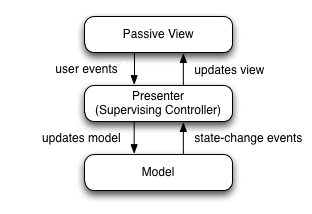
\includegraphics{../images/Model_View_Presenter_GUI_Design_Pattern.png}
  \caption{mvp}
\end{figure}

Hình 7: Kiến trúc MVP

Ở đây, ta thấy điểm yếu View-Controller nhập nhằng của MVC được khắc
phục, khi View kiêm luôn việc nhận tương tác. Đồng thời, Model và View
hoàn toàn không biết nhau, đúng theo nguyên lý tách lớp của Clean
Architecture.

Ta xét một ứng dụng ToDo đơn giản, trong đó các công việc có thể được
đánh dấu đã hoàn thành. Trong ứng dụng, màn hình hiển thị số việc đã và
chưa hoàn thành. Trong màn hình đó, tương tác của MVP như sau:

\begin{enumerate}
  \def\labelenumi{\arabic{enumi}.}
  
  \item
        Presenter lấy tất cả công việc trong Model
  \item
        Presenter đếm số việc hoàn thành, chưa hoàn thành
  \item
        Presenter gọi hàm của View, truyền hai số đếm được ở trên vào
\end{enumerate}

Đến đây, thiết kế đã khá hoàn chỉnh. MVVM chỉ còn cải tiến thêm một điểm
nữa.

\hypertarget{mvvm-model---view---view-model}{%
  \subparagraph{2.3.1.3. MVVM: Model - View - View
    Model}\label{mvvm-model---view---view-model}}

\begin{figure}
  \centering
  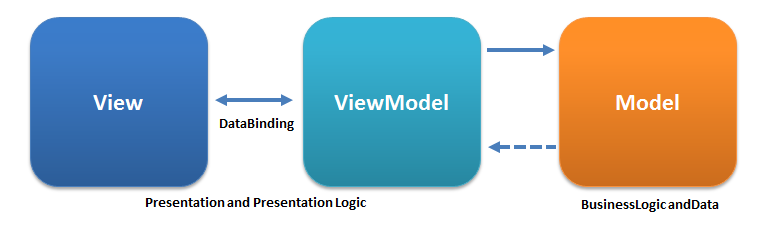
\includegraphics{../images/MVVMPattern.png}
  \caption{mvvm}
\end{figure}

Hình 8: Kiến trúc MVVM

Ta quay về chủ đề chính: MVVM. MVVM giống MVP ở chỗ View Model (từ đây
gọi tắt là VM) kết nối View và Model như Presenter. Điểm khác biệt là
cách truyền dữ liệu:

\begin{itemize}
  
  \item
        Trong MVP, Presenter gọi hàm của View để truyền dữ liệu cho View
  \item
        Trong MVVM, VM dùng \emph{data binding} để truyền dữ liệu cho View
\end{itemize}

Data binding là cơ chế để \emph{tự động} đưa dữ liệu vào thành phần hiển
thị. Quay lại ví dụ ToDo ở trên, nếu dùng data binding để ``gắn'' (bind)
danh sách công việc vào View, thì khi danh sách thay đổi, View cũng tự
động thay đổi theo.

Do dùng data binding thay vì gọi hàm thủ công, VM không cần có tham
chiếu tới View, khác với Presenter. Điều này giúp liên kết View - VM
thêm \emph{lỏng lẻo} (loose coupling), giúp kiểm thử dễ dàng hơn. Phần
còn lại của hai mô hình giống nhau: View cần biết VM để chuyển tương
tác; VM cần biết Model để lấy dữ liệu.

Do là mô hình phù hợp nhất trong cả ba với riêng Android, MVVM được chọn
làm nền tảng cho Kiến trúc Google khuyên dùng.

\hypertarget{kiux1ebfn-truxfac-google-khuyuxean-duxf9ng}{%
  \paragraph{\texorpdfstring{2.3.2. Kiến trúc Google khuyên dùng
    }{2.3.2. Kiến trúc Google khuyên dùng }}\label{kiux1ebfn-truxfac-google-khuyuxean-duxf9ng}}

Kiến trúc Google khuyên dùng có gốc là mô hình MVVM, có dạng như sau:

\begin{figure}
  \centering
  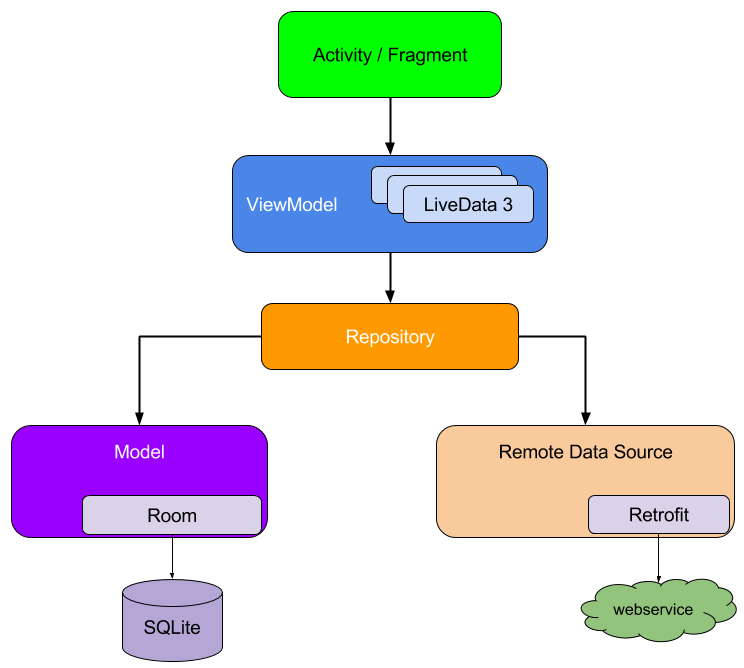
\includegraphics{../images/final-architecture.png}
  \caption{Google recommended architecture}
\end{figure}

Hình 9: Kiến trúc Google khuyên dùng

\begin{itemize}
  
  \item
        Repository là Model trong MVVM, giúp VM lấy dữ liệu mà không cần quan
        tâm dữ liệu lấy từ đâu: cơ sở dữ liệu, gọi API qua mạng,\ldots{}
  \item
        LiveData là cơ chế data binding dùng luồng dữ liệu (stream)
  \item
        Activity/Fragment là View
\end{itemize}

Repository là một điểm được chi tiết hóa so với MVVM. Google cho rằng
một ứng dụng không nên hoàn toàn vô dụng nếu không có mạng. Do đó, cần
có hai nguồn dữ liệu: dữ liệu từ máy chủ, và dữ liệu đệm, ngoại tuyến.
Khi có nhiều nguồn dữ liệu, mẫu thiết kế Repository là lựa chọn hiển
nhiên để trừu tượng hóa chúng.

yacv sử dụng kiến trúc này, dù không có tính năng liên quan đến mạng. Lý
do là yacv có tính năng quét truyện hoạt động chậm giống như giao tiếp
mạng, nên cần dữ liệu đệm và dữ liệu quét thực tế.

\hypertarget{sqlite}{%
  \subsubsection{\texorpdfstring{2.4. SQLite
    }{2.4. SQLite }}\label{sqlite}}

SQLite là một hệ quản trị cơ sở dữ liệu quan hệ (RDBMS). Từ ``Lite''
trong tên có nghĩa là ``nhỏ'', thể hiện mục tiêu thiết kế chính của nó
là nhỏ gọn. SQLite có thể được nhúng vào phần mềm khác ở dạng thư viện,
thay vì là một phần mềm riêng với cấu trúc chủ-khách như MySQL,\ldots{}
Ngay từ những phiên bản đầu, Android đã tích hợp SQLite, giúp lập trình
viên không phải nhúng SQLite vào từng ứng dụng.

Để đạt mục tiêu, SQLite chỉ giữ các tính năng SQL cốt lõi
(tạo/đọc/sửa/xóa), giao dịch (có ACID), và chỉ tối ưu cho việc truy cập
từ một ứng dụng cùng lúc. Các tính năng thường có trong RDBMS cho máy
chủ, như nhân bản (replication), chia dữ liệu tự động (sharding), khóa
dòng, đọc ghi nhiều luồng cùng lúc,\ldots{} được loại bỏ. Do đó, với nhu
cầu lưu trữ đơn giản, SQLite vừa nhanh vừa gọn.

yacv dùng SQLite để lưu đệm thông tin truyện, tránh việc phải quét nhiều
lần.

\hypertarget{room}{%
  \paragraph{\texorpdfstring{2.4.1. Room }{2.4.1. Room }}\label{room}}

Room là một thư viện thuộc Jetpack, giúp lập trình viên dùng SQLite tốt
hơn. Đây có thể xem là một thư viện ORM đơn giản cho SQLite. Room tự
động làm nhiều công việc liên quan đến SQL:

\begin{itemize}
  
  \item
        Tạo bảng: Lập trình viên chỉ cần khai báo các đối tượng dữ liệu như
        một lớp hướng đối tượng thông thường, rồi đánh dấu với Annotation và
        interface của Room. Sau đó, Room sinh các bảng tương ứng.
  \item
        Truy vấn: Lập trình viên chỉ cần viết câu lệnh SQL. Sau đó, Room sinh
        hàm truy vấn tương ứng, chuyển dữ liệu dạng đối tượng sang dạng để lưu
        trong bảng và ngược lại.
  \item
        Kiểm tra truy vấn khi biên dịch: lỗi lệnh SQL có thể được dò ra ngay
        khi biên dịch chứ không cần chờ đến khi chạy.
  \item
        Kiểm soát lược đồ (schema): Khi thêm/sửa/xóa bảng/cột, Room luôn phát
        hiện và ép lập trình viên viết cơ chế cập nhật. Do đó, ứng dụng dùng
        lược đồ cũ khi được cập nhật sẽ biết cách sửa cơ sở dữ liệu đến phiên
        bản lược đồ mới.
  \item
        Tương thích với LiveData: Room cho phép View cập nhật dữ liệu theo cơ
        sở dữ liệu chỉ bằng vài dòng mã dùng LiveData.
\end{itemize}

\hypertarget{tuxecm-kiux1ebfm-vux103n-bux1ea3n}{%
  \paragraph{\texorpdfstring{2.4.2. Tìm kiếm văn bản
    }{2.4.2. Tìm kiếm văn bản }}\label{tuxecm-kiux1ebfm-vux103n-bux1ea3n}}

Tìm kiếm văn bản (full-text search, hay gọi tắt là FTS) là một trong số
ít các tính năng nâng cao được giữ lại trong SQLite. Cũng như các thư
viện tìm kiếm khác, SQLite cài đặt chức năng này bằng chỉ mục đảo
(inverted index):

\begin{enumerate}
  \def\labelenumi{\arabic{enumi}.}
  
  \item
        Khi dữ liệu văn bản được ghi, nó được tách thành các từ.
  \item
        Các từ được đưa vào từ điển, với khóa là chính từ đó, còn giá trị là
        ID của hàng \texttt{rowid}.
\end{enumerate}

FTS khác với đánh chỉ mục thường (cũng là chỉ mục đảo nhưng cho kiểu dữ
liệu thông thường) ở bước 1: \emph{từng từ} được tách ra, còn chỉ mục
thường dùng \emph{cả} văn bản. Do đó, khi tìm từ lẻ, FTS có thể tìm các
hàng chứa từ đó rất nhanh. Điểm yếu là ghi chậm, kích cỡ lớn hơn chỉ mục
thường. Nếu bản thân dữ liệu văn bản trong cột là một khối, ví dụ như
email, chỉ mục thường đã đủ tốt, không cần FTS.

Trong SQLite, một số kĩ thuật xử lí ngôn ngữ tự nhiên cơ bản cũng được
áp dụng trong bước 1, như rút gọn từ (stemming, dùng thuật toán Porter,
ví dụ khi tìm ``run'' sẽ ra được cả ``runs'', ``running'', ``ran''; tất
nhiên chỉ đúng với tiếng Anh), giúp kết quả tìm kiếm linh động hơn.

yacv có tính năng tìm kiếm liên quan đến tiêu đề, tên nhân vật,\ldots{}
đều là những câu văn, đoạn văn. Do đó, FTS có vai trò không thể thiếu để
tăng tốc tìm kiếm trong ứng dụng.

\hypertarget{ux111ux1ecbnh-dux1ea1ng-tux1ec7p-nuxe9n-.zip-vuxe0-.cbz}{%
  \subsubsection{\texorpdfstring{2.5. Định dạng tệp nén \texttt{.zip} và
      \texttt{.cbz}
    }{2.5. Định dạng tệp nén .zip và .cbz }}\label{ux111ux1ecbnh-dux1ea1ng-tux1ec7p-nuxe9n-.zip-vuxe0-.cbz}}

Các tệp truyện mà yacv đọc có định dạng \texttt{.cbz}, về bản chất chính
là tệp nén \texttt{.zip} thông thường. Do yêu cầu của các phần sau, định
dạng tệp \texttt{.zip} cũng cần được trình bày ở mức cơ bản.

\hypertarget{ux111ux1ecbnh-dux1ea1ng-tux1ec7p-nuxe9n-.zip}{%
  \paragraph{\texorpdfstring{2.5.1. Định dạng tệp nén
      \texttt{.zip}}{2.5.1. Định dạng tệp nén .zip}}\label{ux111ux1ecbnh-dux1ea1ng-tux1ec7p-nuxe9n-.zip}}

ZIP là định dạng tệp nén không mất mát (lossless). Được phát minh vào
năm 1989 bởi Phil Katz, ZIP đã trở thành định dạng nén tiêu chuẩn, được
hỗ trợ trên gần như mọi nền tảng, bao gồm Android.

ZIP thực chất là một định dạng chứa (container), chuyên chứa dữ liệu
nén, chứ không phải thuật toán nén; thuật toán nén hay dùng nhất trong
ZIP là DEFLATE. Một trong các mục tiêu của ZIP là giúp việc sửa tệp nén
(thêm, sửa, xóa tệp con trong tệp ZIP) nhanh nhất có thể. Mục tiêu đó
thể hiện ở thiết kế sau:

\begin{itemize}
  
  \item
        Thuật toán nén mỗi tệp gốc thành một tệp nhị phân, ở đây gọi là
        \emph{tệp nén lẻ} (data trong Hình 10). Sau đó, các tệp nén lẻ này
        được nối thành tệp ZIP cuối cùng.
  \item
        Trước mỗi tệp nén lẻ là một header gọi là \emph{File Entry} để lưu
        thông tin liên quan.
  \item
        Ở \emph{cuối} tệp ZIP, sau khi đã nối các tệp nén lẻ và header lại,
        các header được gom lại, lưu một lần nữa vào một cấu trúc gọi là
        \emph{Central Directory}. Có thể so sánh File Entry như các \emph{đề
          mục}, còn Central Directory là \emph{mục lục}.
  \item
        Hai thông tin quan trọng trong File Entry là tên tệp gốc và \emph{vị
          trí bắt đầu} (offset), tức số byte tính từ đầu tệp ZIP đến tệp nén lẻ
        tương ứng.
\end{itemize}

\begin{figure}
  \centering
  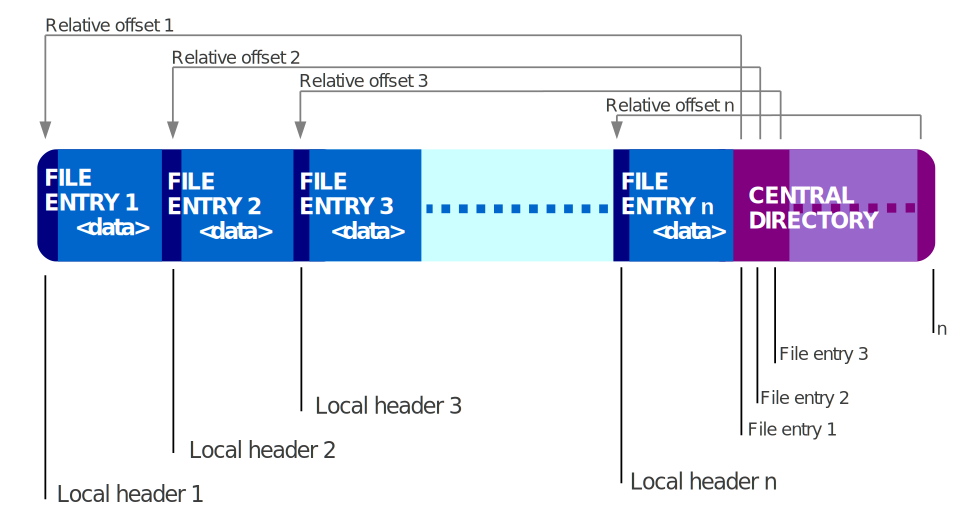
\includegraphics{../images/ZIP-64_Internal_Layout.svg}
  \caption{zip file layout}
\end{figure}

Hình 10: Cấu trúc tệp nén ZIP

Ta phân tích kĩ hơn:

\begin{itemize}
  \item
        Do từng tệp được nén riêng, có thể dùng thuật toán khác nhau cho hiệu
        quả tốt với từng tệp.
  \item
        Cũng do nén riêng, việc thêm/sửa/xóa (gọi chung là sửa) và giải nén có
        thể được thực hiện với từng tệp nén lẻ, thay vì phải giải nén, sửa,
        rồi nén lại toàn bộ.
  \item
        Nhờ mục lục (chứa vị trí tệp nén lẻ), việc sửa còn diễn ra nhanh do
        ứng dụng biết vị trí để đọc ghi dữ liệu.
  \item
        Mục lục đặt ở cuối là tối ưu:

        \begin{itemize}
          
          \item
                Giả sử mục lục đặt ở đầu. Khi sửa, toàn bộ các tệp nén lẻ phải di
                chuyển để tạo chỗ cho mục lục mới (giống như thêm một phần tử vào
                mảng ở vị trí đầu: toàn bộ các phần tử sau bị đẩy lên để tạo chỗ
                trống).
          \item
                Do mục lục nằm ở cuối tệp tin, khi sửa tệp nén, chỉ cần đẩy các tệp
                nén lẻ từ chỗ sửa. Đây có thể coi là một tối ưu nhỏ, nhưng trước đây
                là một điểm sáng. Do đĩa mềm - phương tiện chia sẻ chủ yếu thời đó -
                có dung lượng nhỏ, tệp ZIP có thể phải cắt ra cho vừa. Cách sửa tệp
                linh động này cho phép chỉ ghi lại dữ liệu ở một số đĩa mềm, thay vì
                ghi lại toàn bộ.
          \item
                Hơn nữa, nếu mục lục ở đầu thì ngay trong khi nén, các tệp nén lẻ bị
                di chuyển như trên do mục lục liên tục được cập nhật.
        \end{itemize}
\end{itemize}

Tóm lại, cấu trúc tệp nén ZIP cho phép sửa và giải nén từng tệp gốc rất
dễ dàng. Nhiều định dạng tệp nén khác (TAR, 7z,\ldots) không có tính
năng này, do gộp toàn bộ các tệp vào rồi nén một thể. Trong trường hợp
đó, tệp nén được gọi là \emph{đặc} (solid), và rất khó để đọc/sửa tệp
lẻ.

\hypertarget{ux111ux1ecbnh-dux1ea1ng-tux1ec7p-truyux1ec7n-.cbz}{%
  \paragraph{\texorpdfstring{2.5.2. Định dạng tệp truyện
      \texttt{.cbz}}{2.5.2. Định dạng tệp truyện .cbz}}\label{ux111ux1ecbnh-dux1ea1ng-tux1ec7p-truyux1ec7n-.cbz}}

Tệp truyện CBZ chỉ là một tệp nén ZIP thông thường, trong đó có:

\begin{itemize}
  
  \item
        Các tệp ảnh trang truyện: Các tệp này có tên được đánh số tăng dần để
        biểu thị thứ tự trang.
  \item
        (Tùy chọn) Một tệp metadata: Có nhiều định dạng metadata. Hiện nay,
        yacv chấp nhận định dạng ComicInfo, được trình bày ở
        \protect\hyperlink{P8.2-comicinfo.xsd}{Phụ lục 2}.
\end{itemize}

\begin{center}\rule{0.5\linewidth}{0.5pt}\end{center}

\hypertarget{chux1b0ux1a1ng-3-phuxe2n-tuxedch-yuxeau-cux1ea7u-thiux1ebft-kux1ebf}{%
  \subsection{\texorpdfstring{3. Chương 3: Phân tích yêu cầu \& Thiết kế
    }{3. Chương 3: Phân tích yêu cầu \& Thiết kế }}\label{chux1b0ux1a1ng-3-phuxe2n-tuxedch-yuxeau-cux1ea7u-thiux1ebft-kux1ebf}}

Chương này phân tích yêu cầu để lập ra đặc tả yêu cầu, là bộ khung cho
quá trình phát triển ứng dụng.

\hypertarget{muxf4-tux1ea3-chung}{%
  \subsubsection{\texorpdfstring{3.1. Mô tả chung
    }{3.1. Mô tả chung }}\label{muxf4-tux1ea3-chung}}

\hypertarget{ngux1b0ux1eddi-duxf9ng}{%
  \paragraph{\texorpdfstring{3.1.1. Người dùng
    }{3.1.1. Người dùng }}\label{ngux1b0ux1eddi-duxf9ng}}

Ứng dụng yacv tập trung vào một số ít người dùng, là một trong hai nhóm
sau:

\begin{itemize}
  
  \item
        Người dùng sưu tầm truyện
  \item
        Người dùng có yêu cầu đọc truyện với chất lượng hình ảnh cao
\end{itemize}

Cả hai nhóm có điểm chung là kĩ tính, yêu cầu cao về trải nghiệm đọc
truyện, cụ thể là về \emph{chất lượng hình ảnh}. Cũng do kĩ tính, nên cả
hai nhóm không cần nhiều chức năng, tuy nhiên có yêu cầu cao về từng
chức năng. Nhóm người dùng sưu tầm truyện còn có yêu cầu về \emph{xem
  thông tin (metadata)} của tệp truyện.

\hypertarget{mux1ee5c-ux111uxedch}{%
  \paragraph{\texorpdfstring{3.1.2. Mục đích
    }{3.1.2. Mục đích }}\label{mux1ee5c-ux111uxedch}}

Trước khi đi vào chi tiết yêu cầu ở mục tiếp theo, tôi muốn làm rõ mục
đích của sản phẩm đã nhắc ở \protect\hyperlink{P1.1-background}{mục
  1.1}.

\begin{itemize}
  
  \item
        Ứng dụng yacv chỉ bao gồm các tính năng liên quan đến đọc
        \textbf{truyện tranh} ngoại tuyến (tức đọc các tệp truyện có sẵn trên
        điện thoại người dùng).
  \item
        Ứng dụng \emph{không phải} là ứng dụng khách cho các trang đọc truyện
        hiện có, hay có máy chủ tập trung riêng để cung cấp truyện.
  \item
        Ứng dụng \emph{không có} khả năng đọc truyện đuôi \texttt{.pdf}, cùng
        với các định dạng truyện thiên về chữ khác như \texttt{.txt},
        \texttt{.epub}.
\end{itemize}

Các giới hạn này nhằm tránh cho phần mềm quá phức tạp với tôi, đồng thời
phù hợp (không thừa thiếu chức năng) so với nhu cầu của nhóm người dùng
mục tiêu đã nêu ở \protect\hyperlink{P3.1.1-users}{mục 3.1.1}.

\hypertarget{yuxeau-cux1ea7u-ux111ux1eb7t-ra}{%
  \subsubsection{\texorpdfstring{3.2. Yêu cầu đặt ra
    }{3.2. Yêu cầu đặt ra }}\label{yuxeau-cux1ea7u-ux111ux1eb7t-ra}}

\hypertarget{yuxeau-cux1ea7u-chux1ee9c-nux103ng}{%
  \paragraph{\texorpdfstring{3.2.1. Yêu cầu chức năng
    }{3.2.1. Yêu cầu chức năng }}\label{yuxeau-cux1ea7u-chux1ee9c-nux103ng}}

Ứng dụng có các chức năng chính sau:

\begin{itemize}
  
  \item
        Quét các tệp truyện trên thiết bị
  \item
        Hiển thị danh sách truyện
  \item
        Đọc truyện
  \item
        Xem metadata truyện
  \item
        Tìm kiếm truyện
  \item
        Xóa truyện
\end{itemize}

\hypertarget{yuxeau-cux1ea7u-phi-chux1ee9c-nux103ng}{%
  \paragraph{\texorpdfstring{3.2.2. Yêu cầu phi chức năng
    }{3.2.2. Yêu cầu phi chức năng }}\label{yuxeau-cux1ea7u-phi-chux1ee9c-nux103ng}}

Ứng dụng cần đạt một số tiêu chí sau:

\begin{itemize}
  \item
        Phản hồi nhanh: Các thao tác cần có thời gian phản hồi nhanh. Phản hồi
        nhanh không nhất thiết là thời gian thực thi ngắn, mà là luôn có các
        thông báo tiến độ cho người dùng.

        \begin{itemize}
          
          \item
                Luôn hiện thông báo chờ khi làm việc gì đó lâu
          \item
                Nếu có nhiều kết quả tìm kiếm, hiển thị từ từ, đưa kết quả đã biết
                lên trước
        \end{itemize}
  \item
        Tốc độ xem truyện chấp nhận được: Đây là một phần của phản hồi nhanh,
        nhưng được tách riêng vì độ quan trọng của nó. Tốc độ xem truyện gồm
        hai tiêu chí:

        \begin{itemize}
          
          \item
                Tốc độ mở truyện, tức tốc độ xem trang đầu (có thể so với first
                contentful paint trong lập trình web)
          \item
                Tốc độ cuộn trang tới-lui
        \end{itemize}
  \item
        Chiếm ít bộ nhớ: Bộ nhớ chiếm dụng của ứng dụng gồm hai phần: bộ nhớ
        RAM và bộ nhớ tạm, cả hai cần sử dụng ít dung lượng nhất có thể. Đây
        là một yêu cầu đáng cân nhắc, lí do vì kích cỡ từng tệp truyện thường
        rất lớn (từ vài chục đến hơn một trăm megabyte), tuy nhiên cần chú ý
        cân bằng yêu cầu này với yêu cầu về tốc độ (đánh đổi không gian-thời
        gian).
  \item
        Giao diện đơn giản, trực quan: Người dùng hướng đến có thể xếp vào
        nhóm người dùng ``say mê'' (enthusiast), do đó giao diện chỉ cần đơn
        giản rõ ràng, không màu mè, tập trung vào tính năng.
\end{itemize}

\hypertarget{phuxe2n-tuxedch-yuxeau-cux1ea7u}{%
  \subsubsection{\texorpdfstring{3.3 Phân tích yêu cầu
    }{3.3 Phân tích yêu cầu }}\label{phuxe2n-tuxedch-yuxeau-cux1ea7u}}

Mỗi yêu cầu đã xác định trong
\protect\hyperlink{P3.2.1-functional-requirements}{mục 3.2.1.} được coi
là một ca sử dụng, được trình bày trong các tiểu mục dưới đây.

\emph{Người dùng duy nhất} trong các ca sử dụng là \emph{người đọc}, do
đó hai cụm từ này sẽ được dùng hoán đổi cho nhau. Do ứng dụng hoàn toàn
ngoại tuyến, người đọc cũng không có tương tác với nhau.

Do ứng dụng đơn giản, các ca sử dụng tách biệt, nên mỗi ca sử dụng gắn
với một \emph{màn hình}. Có tổng cộng năm màn hình sẽ được mô tả, gồm:

\begin{itemize}
  
  \item
        Màn hình Thư viện
  \item
        Màn hình Thư mục
  \item
        Màn hình Đọc truyện
  \item
        Màn hình Metadata
  \item
        Màn hình Tìm kiếm
\end{itemize}

\hypertarget{quuxe9t-cuxe1c-tux1ec7p-truyux1ec7n-truxean-thiux1ebft-bux1ecb}{%
  \paragraph{\texorpdfstring{3.3.1. Quét các tệp truyện trên thiết bị
    }{3.3.1. Quét các tệp truyện trên thiết bị }}\label{quuxe9t-cuxe1c-tux1ec7p-truyux1ec7n-truxean-thiux1ebft-bux1ecb}}

\begin{itemize}
  \item
        \textbf{Mô tả}:

        Người đọc \emph{chọn} một thư mục trong điện thoại làm thư mục gốc.
        Ứng dụng sẽ \emph{quét} thư mục này và tìm các tệp truyện, rồi hiển
        thị những thư mục chứa tệp truyện cho người đọc chọn.
  \item
        \textbf{Luồng chính}:

        \begin{enumerate}
          \def\labelenumi{\arabic{enumi}.}
          
          \item
                Người đọc bật ứng dụng (tức ở Màn hình Thư viện)
          \item
                Người đọc ấn vào nút thay đổi thư mục gốc.
          \item
                Trình chọn thư mục của Android hiện ra, cho phép người đọc chọn thư
                mục làm thư mục gốc.
          \item
                Màn hình Thư viện trở lại, quét và hiển thị các thư mục chứa truyện
                trong thư mục gốc.
        \end{enumerate}
  \item
        \textbf{Luồng thay thế}:

        Nếu người đọc đã chọn một thư mục gốc, ca sử dụng này \emph{thay thế}
        thư mục gốc đã chọn bằng thư mục vừa chọn.

        Nếu người đọc không chọn thư mục, quay lại Màn hình Thư viện.
  \item
        \textbf{Luồng ngoại lệ}:

        Nếu có lỗi trong quá trình chọn thư mục, cần gợi ý người đọc chọn lại.
        Lỗi gồm:

        \begin{itemize}
          
          \item
                Thiếu quyền
          \item
                Không tìm được thư mục gốc
          \item
                Thư mục gốc không có truyện
        \end{itemize}

        Nếu có lỗi trong quá trình quét cần phải giảm thiểu và giấu khỏi người
        đọc.
  \item
        \textbf{Điều kiện}:

        \begin{itemize}
          \item
                Tiền điều kiện: Ứng dụng ở Màn hình Thư viện
          \item
                Hậu điều kiện: Ứng dụng ở Màn hình Thư viện

                \begin{itemize}
                  
                  \item
                        Hiển thị thư mục truyện quét được
                  \item
                        Hiển thị lỗi nếu có (ba loại lỗi ở trên)
                \end{itemize}
        \end{itemize}
  \item
        \textbf{Yêu cầu phi chức năng}:

        Nếu đang quét, Màn hình Thư viện cần hiển thị danh sách thư mục theo
        tiến độ, ứng dụng quét đến đâu hiển thị đến đấy.

        Mỗi thư mục cần hiển thị:

        \begin{itemize}
          
          \item
                Tên thư mục
          \item
                Ảnh đại diện cho thư mục: bìa một truyện bất kì tìm được trong thư
                mục
        \end{itemize}
\end{itemize}

Đây là ca sử dụng đầu tiên khi người đọc khởi động ứng dụng lần đầu. Các
tệp truyện sẽ được quét từ thư mục gốc, rồi được gom lại theo thư mục
theo mô tả ở \protect\hyperlink{P3.3.2-show-library}{ca sử dụng tiếp
  theo}.

Màn hình đầu tiên khi người đọc bật lên gọi là \emph{Màn hình Thư viện}
(Library screen). Các thư mục chứa truyện, hoặc thông báo lỗi liên quan
đến bản thân quá trình chọn truyện (đã miêu tả trong bước 6 ở trên) sẽ
được hiển thị ở màn hình này.

Khi quét, ứng dụng phải đọc luôn cả metadata của tệp truyện nếu có. Các
trường trong metadata được giải thích chi tiết trong
\protect\hyperlink{P8.1-metadata}{Phụ lục 1}. Hiện nay, yacv chấp nhận
định dạng metadata ComicInfo, là một tệp XML trong tệp truyện.
\protect\hyperlink{P8.2-comicinfo.xsd}{Phụ lục 2} trình bày lược đồ XSD
của định dạng metadata này.

Một số metadata có thể được trích xuất ngay từ tên tệp truyện. Do không
có quy chuẩn trong việc đặt tên tệp, cách trích xuất này không ổn định,
tuy nhiên cũng không phải ý tưởng tồi.

\begin{verbatim}
Wolverine 1982(1) #1
│         │       └─ Number/no (String): issue number, ~ chapter. Note that it is a String.
│         └─ Volume (Int): Several series can have the same name, so they are distinguished by either year or version.
└─Series (String): Name of the series.
Count (Int): number of issues (Not in the example).
\end{verbatim}

Tới đây người đọc có thể thực hiện các ca sử dụng khác, trong đó quan
trọng nhất là duyệt theo thư mục rồi xem truyện.

\hypertarget{hiux1ec3n-thux1ecb-danh-suxe1ch-truyux1ec7n}{%
  \paragraph{\texorpdfstring{3.3.2. Hiển thị danh sách truyện
    }{3.3.2. Hiển thị danh sách truyện }}\label{hiux1ec3n-thux1ecb-danh-suxe1ch-truyux1ec7n}}

\begin{itemize}
  \item
        \textbf{Mô tả}:

        Người đọc duyệt truyện theo thư mục, rồi chọn truyện và xem.
  \item
        \textbf{Luồng chính}:

        \begin{enumerate}
          \def\labelenumi{\arabic{enumi}.}
          
          \item
                Người đọc bật ứng dụng (tức ở Màn hình Thư viện), có danh sách
                truyện (tức đã chọn thư mục gốc và quét được ít nhất một thư mục
                chứa truyện).
          \item
                Người đọc chọn một thư mục.
          \item
                Ứng dụng chuyển sang Màn hình Thư mục, hiển thị \emph{danh sách
                  truyện} trong thư mục đó cho người đọc xem và chọn.
        \end{enumerate}
  \item
        \textbf{Điều kiện}:

        \begin{itemize}
          \item
                Tiền điều kiện:

                \begin{itemize}
                  
                  \item
                        Ứng dụng ở Màn hình Thư viện
                  \item
                        Đã chọn thư mục gốc và đã quét được ít nhất một thư mục chứa
                        truyện
                \end{itemize}
          \item
                Hậu điều kiện: Ứng dụng ở Màn hình Thư mục.
        \end{itemize}
  \item
        \textbf{Yêu cầu phi chức năng}:

        Nếu đang quét, màn hình Thư mục cần hiển thị danh sách truyện theo
        tiến độ, ứng dụng quét đến đâu hiển thị đến đấy.

        Mỗi truyện cần hiển thị:

        \begin{itemize}
          
          \item
                Tên truyện
          \item
                Bìa truyện
          \item
                Tiến độ đọc
          \item
                Đánh giá yêu thích
        \end{itemize}
\end{itemize}

Đây là một trong hai ca sử dụng chính của ứng dụng, bên cạnh (và là tiền
điều kiện cho) \protect\hyperlink{P3.3.3-read-comic}{ca sử dụng đọc
  truyện} sẽ được miêu tả tiếp theo.

Màn hình khi người đọc chọn một thư mục gọi là \emph{Màn hình Thư mục}
(Directory screen). Cũng giống như Màn hình Thư viện, ảnh bìa và tên của
truyện được hiển thị để người đọc chọn.

Trong yacv, truyện được quản lí và duyệt theo thư mục. Có hai lí do cho
lựa chọn thiết kế này:

\begin{itemize}
  \item
        Giảm độ phức tạp khi lập trình
  \item
        Các phương pháp duyệt khác không trực quan

        \begin{itemize}
          
          \item
                Các phương pháp duyệt khác chỉ bao gồm duyệt theo metadata, tức
                duyệt theo các thông tin đi kèm như Tác giả, Nhân vật, Bộ
                truyện,\ldots{} thì yêu cầu truyện phải có đủ metadata. Trên thực
                tế, không phải tệp truyện nào cũng có đủ thông tin này, do vậy sẽ có
                trường hợp rất nhiều truyện bị gom vào mục ``Không đủ thông tin''.
                Hơn nữa, giả sử truyện có đi kèm metadata, ta xem xét tiếp trường
                hợp dưới.
          \item
                Giả sử ta quản lí theo Nhân vật: Vậy để trực quan, yacv phải hiển
                thị ảnh nhân vật. Hiện nay, việc nhận diện và cắt đúng ảnh phần mặt
                nhân vật ra để tạo ảnh đại diện có thể nói là bất khả thi. Do vậy,
                khi duyệt theo Nhân vật, người đọc chỉ có thể thấy tên, không thấy
                một hình ảnh gợi ý nào khác, dẫn đến khó khăn khi sử dụng. Lập luận
                tương tự có thể dùng với các cách xếp khác.
          \item
                Một cách xếp có thể nói là tốt là xếp theo Bộ truyện, tuy nhiên ta
                lại quay về vấn đề thiếu metada.
        \end{itemize}
\end{itemize}

Hơn nữa, các thư mục cần được ``làm phẳng''. ``Làm phẳng'' có nghĩa là
hiển thị thư mục con (cháu,\ldots) ngang hàng với thư mục gốc. Ví dụ sau
cho thấy cách yacv làm phẳng cây thư mục:

\begin{verbatim}
| Cây thư mục gốc                   | yacv đã làm phẳng         |
|-----------------------------------|---------------------------|
| thư mục gốc                       | thư mục gốc               |
| ├── Original Sin #1.cbz           | └── Original Sin #1.cbz   |
| └── House of M                    | House of M                |
|     ├── House of M #1.cbz         | ├── House of M #1.cbz     |
|     ├── House of M #3.cbz         | └── House of M #3.cbz     |
|     └── Tie-ins                   | Tie-ins                   |
|         └── Black Panther #7.cbz  | └── Black Panther #7.cbz  |
\end{verbatim}

Bảng 3: Cách yacv làm phẳng thư mục

Theo như cột phải Bảng 3, các màn hình trong yacv được tổ chức như sau:

\begin{itemize}
  \item
        Màn hình Thư viện: có 3 thư mục:

        \begin{itemize}
          
          \item
                thư mục gốc
          \item
                House of M
          \item
                Tie-ins
        \end{itemize}
  \item
        Khi chọn ``House of M'': chuyển sang Màn hình Thư mục tương ứng, không
        có thư mục con, và có 2 tệp truyện:

        \begin{itemize}
          
          \item
                House of M \#1.cbz
          \item
                House of M \#3.cbz
        \end{itemize}
  \item
        Tương tự với các thư mục khác.
\end{itemize}

Có ba lí do cho lựa chọn thiết kế này:

\begin{itemize}
  \item
        Giảm độ phức tạp khi lập trình.
  \item
        Người đọc không phải đi qua nhiều tầng thư mục để đến được tệp truyện
        cần đọc.
  \item
        Không có ca sử dụng có ý nghĩa cho thư mục lồng nhau:

        Trường hợp hợp lí nhất cho việc có thư mục lồng nhau là khi lưu các
        tệp truyện liên quan đến một bộ truyện (tie-ins), như cột trái Bảng 3:

        \begin{itemize}
          
          \item
                Thư mục cha (House of M) chứa tệp truyện trong bộ truyện cùng tên và
                thư mục tie-ins.
          \item
                Thư mục Tie-ins chứa các tệp truyện tie-in.
        \end{itemize}

        Tuy nhiên, bản thân các tệp tie-in lại là tệp truyện thông thường
        trong một bộ truyện khác, do đó nếu tổ chức thư mục như thế này sẽ dẫn
        đến tình trạng lặp tệp truyện, là điều không mong muốn ngay cả với máy
        tính.
\end{itemize}

\hypertarget{ux111ux1ecdc-truyux1ec7n}{%
  \paragraph{\texorpdfstring{3.3.3. Đọc truyện
    }{3.3.3. Đọc truyện }}\label{ux111ux1ecdc-truyux1ec7n}}

\begin{itemize}
  \item
        \textbf{Mô tả}:

        Người đọc chọn một truyện để xem.
  \item
        \textbf{Luồng chính}:

        \begin{enumerate}
          \def\labelenumi{\arabic{enumi}.}
          
          \item
                Người đọc bật ứng dụng, đã chọn thư mục gốc, đã quét được ít nhất
                một thư mục chứa truyện, đã chọn một thư mục (tức ở Màn hình Thư
                mục).
          \item
                Ứng dụng hiển thị danh sách truyện trong thư mục đó cho người đọc
                xem và chọn.
          \item
                Người đọc chọn một truyện và đọc.
          \item
                Màn hình Đọc truyện hiển thị trang truyện cho người đọc.
          \item
                Người đọc vuốt qua lại theo phương ngang để chuyển trang.
        \end{enumerate}
  \item
        \textbf{Luồng thay thế}:

        Xem phần Màn hình Tìm kiếm. Màn hình Đọc truyện có thể được kích hoạt
        bằng cách ấn vào truyện hiển thị trong màn hình này.
  \item
        \textbf{Luồng ngoại lệ}:

        Nếu tệp truyện không tìm thấy được, báo cho người đọc và giữ nguyên ở
        Màn hình Thư mục.
  \item
        \textbf{Điều kiện}:

        \begin{itemize}
          
          \item
                Tiền điều kiện: Ứng dụng ở Màn hình Thư mục.
          \item
                Hậu điều kiện: Ứng dụng ở Màn hình Đọc truyện.
        \end{itemize}
  \item
        \textbf{Yêu cầu phi chức năng}:

        \begin{itemize}
          
          \item
                Nếu người đọc đã đọc truyện, ứng dụng cần đưa về chính trang truyện
                đang đọc dở. Nếu đã đọc đến trang cuối, tức đã đọc xong, ứng dụng
                cần đưa về trang đầu tiên.
          \item
                Trải nghiệm cuộn trang mượt mà nhất có thể.
        \end{itemize}
\end{itemize}

Đây là một trong hai ca sử dụng chính của ứng dụng, bên cạnh (và là mục
đích của) \protect\hyperlink{P3.3.2-show-library}{ca sử dụng hiển thị
  danh sách truyện} đã được miêu tả ở trên.

Màn hình khi người đọc đọc một truyện gọi là \emph{Màn hình Đọc truyện}.
Màn hình này cho phép người đọc duyệt các trang truyện theo phương
ngang. Mục tiêu là thiết kế màn hình này sao cho có trải nghiệm gần
giống nhất với ứng dụng Thư viện ảnh (Gallery) tích hợp trong mọi điện
thoại Android.

\hypertarget{xem-metadata-truyux1ec7n}{%
  \paragraph{\texorpdfstring{3.3.4. Xem metadata truyện
    }{3.3.4. Xem metadata truyện }}\label{xem-metadata-truyux1ec7n}}

\begin{itemize}
  \item
        \textbf{Mô tả}:

        Trong Màn hình Đọc truyện, người đọc ấn nút để xem metadata.
  \item
        \textbf{Luồng chính}:

        \begin{enumerate}
          \def\labelenumi{\arabic{enumi}.}
          
          \item
                Người đọc bật ứng dụng, chọn một truyện để vào đến Màn hình Đọc
                truyện.
          \item
                Người đọc ấn nút Xem metadata.
          \item
                Ứng dụng hiển thị mọi metadata, bao gồm cả những trường bị thiếu.
                Ảnh bìa của truyện cũng được hiển thị kèm.
          \item
                Người dùng có thể đánh giá truyện bằng nút Yêu thích trong màn hình
                này, hoặc ngược lại (bỏ đánh giá Yêu thích).
        \end{enumerate}
  \item
        \textbf{Điều kiện}:

        \begin{itemize}
          
          \item
                Tiền điều kiện: Ứng dụng ở Màn hình Đọc truyện.
          \item
                Hậu điều kiện: Ứng dụng ở Màn hình Metadata.
        \end{itemize}
  \item
        \textbf{Yêu cầu phi chức năng}:

        \begin{itemize}
          
          \item
                Màn hình Metadata phải hiển thị ảnh bìa, cùng các metadata của
                truyện
          \item
                Những trường metadata trống phải ghi rõ ``Trống'',
                ``Unknown'',\ldots{}
        \end{itemize}
\end{itemize}

Đây là một ca sử dụng phụ, có thể được kích hoạt khi người dùng đang ở
Màn hình Đọc truyện.

Màn hình khi người đọc xem metadata gọi là \emph{Màn hình Metadata}. Màn
hình này có thể có chức năng sửa metadata, tùy theo tiến độ khóa luận để
xem xét có cài đặt không.

Hệ thống đánh giá của ứng dụng chỉ ở mức cơ bản, gồm duy nhất tính năng
Yêu thích. Tính năng này cũng chỉ phục vụ hai mục đích là thể hiện sự
đánh giá của người dùng và lọc nhanh truyện về mặt thị giác (đã nhắc đến
trong phần Mô tả từng bước của
\protect\hyperlink{P3.3.2-show-library}{ca sử dụng hiển thị danh sách
  truyện}).

Các tính năng nâng cao hơn như gợi ý không xuất hiện, do một số lí do
sau:

\begin{itemize}
  
  \item
        Giảm độ phức tạp khi lập trình.
  \item
        Người dùng không có nhu cầu: nhóm người dùng hướng đến có đặc điểm
        hiểu biết về truyện tranh, do đó việc gợi ý có thể coi là thừa thãi.
  \item
        Thiểu thông tin gợi ý: việc gợi ý chỉ có hiệu quả khi có một cơ sở dữ
        liệu về c��c bộ truyện liên quan, hoặc lựa chọn các truyện liên quan
        của cộng đồng người đọc, trong khi yacv là một ứng dụng hoàn toàn
        ngoại tuyến.
\end{itemize}

\hypertarget{tuxecm-kiux1ebfm-truyux1ec7n}{%
  \paragraph{\texorpdfstring{3.3.5. Tìm kiếm truyện
    }{3.3.5. Tìm kiếm truyện }}\label{tuxecm-kiux1ebfm-truyux1ec7n}}

\begin{itemize}
  \item
        \textbf{Mô tả}:

        Trong Màn hình Thư viện, người đọc ấn nút Tìm kiếm để tìm truyện.
  \item
        \textbf{Luồng chính}:

        \begin{enumerate}
          \def\labelenumi{\arabic{enumi}.}
          
          \item
                Người đọc bật ứng dụng.
          \item
                Người đọc ấn nút Tìm kiếm, và gõ từ khóa cần tìm, và ấn nút Enter.
          \item
                Ứng dụng hiển thị kết quả tìm kiếm theo metadata và tên tệp truyện.
        \end{enumerate}
  \item
        \textbf{Luồng ngoại lệ}:

        Nếu không tìm thấy truyện, ứng dụng cần thông báo ở Màn hình Tìm kiếm.
  \item
        \textbf{Điều kiện}:

        \begin{itemize}
          
          \item
                Tiền điều kiện: Ứng dụng ở Màn hình Thư viện.
          \item
                Hậu điều kiện: Ứng dụng ở Màn hình Tìm kiếm.
        \end{itemize}
  \item
        \textbf{Yêu cầu phi chức năng}:

        \begin{itemize}
          
          \item
                Kết quả tìm kiểm cần được gom theo nhóm dựa vào trường metadata tìm
                thấy được. Nếu không có kết quả, phải báo cho người dùng.
          \item
                Nếu có thể, hiển thị ảnh bìa của truyện.
        \end{itemize}
\end{itemize}

Đây là một ca sử dụng phụ, có thể được kích hoạt khi người dùng đang ở
Màn hình Thư viện.

Màn hình khi người đọc \emph{xem kết quả tìm kiếm} gọi là \emph{Màn hình
  Tìm kiếm}. Màn hình này chỉ hiện ra khi người dùng ấn nút Enter để chính
thức tìm kiếm; cho đến trước lúc đó, ứng dụng vẫn ở Màn hình Thư viện.

Màn hình kết quả phải nhóm kết quả theo trường metadata mà kết quả tìm
thấy được. Lấy ví dụ, người dùng tìm kiếm ``Watchmen'' sẽ nhận được Màn
hình Tìm kiếm gần như sau:

\begin{verbatim}
Truyện
- Watchmen #1.cbz
- Watchmen #2.cbz
Bộ truyện
- Watchmen
\end{verbatim}

Tương tác của người đọc với Màn hình Tìm kiếm trên diễn ra như sau:

\begin{itemize}
  
  \item
        Khi ấn vào một mục trong danh sách ``Truyện'', người đọc được đưa đến
        thẳng Màn hình Đọc truyện của truyện đó (và hiển thị ở trang đọc dở
        như đã mô tả ở trong \protect\hyperlink{P3.3.3-read-comic}{ca sử dụng
          đọc truyện}).
  \item
        Khi ấn vào một mục trong danh sách ``Bộ truyện'', người đọc được đưa
        đến màn hình chứa danh sách những truyện trong bộ truyện đã chọn.
        \emph{Màn hình này cần giống với Màn hình Thư mục}. Sau đó, người dùng
        chọn một truyện để đọc như bình thường.
\end{itemize}

Đây chỉ là ví dụ về một từ khóa có kết quả khi tìm theo tên tệp truyện
và bộ truyện. Các trường metadata khác nếu có kết quả phù hợp cũng sẽ
thể hiện theo hình thức trên.

Chú ý rằng bìa truyện luôn được thể hiện khi có thể. Trong ví dụ trên,
chắc chắn phải có bìa truyện cho mọi mục con trong danh sách ``Truyện''.
Còn mục con của ``Bộ truyện'' thì không, lí do là không có đủ dữ liệu
(không có dữ liệu cho logo, banner,.. của bộ truyện). Tương ứng, không
có dữ liệu hiển thị cho danh sách ``Nhân vật'', ``Tác giả'',\ldots{} Đây
là một hạn chế quan trọng về giao diện mà hiện chưa có cách thiết kế hợp
lý.

Nếu không có kết quả, cần thể hiện rõ cho người dùng biết.

Khi người dùng gõ từ khóa để tìm kiếm, một số thông tin gợi ý tìm kiếm
(từ khóa cũ, từ khóa liên quan) có thể hiện ra; tính năng này tùy theo
tiến độ khóa luận để xem xét có cài đặt không. Chỉ khi người dùng ấn
Enter, quá trình tìm kiếm mới bắt đầu, và hiển thị kết quả, chứ không
hiển thị kết quả theo quá trình người dùng gõ phím. Lí do cho lựa chọn
này như sau:

\begin{itemize}
  
  \item
        Giảm độ phức tạp khi lập trình.
  \item
        Không quá cần thiết: ví dụ, bộ máy tìm kiếm của Google cũng chỉ hiện
        gợi ý khi người dùng nhập từ khóa tìm kiếm, phải đến khi ấn Enter thì
        quá trình tìm kiếm mới diễn ra và kết quả chi tiết được hiển thị.
\end{itemize}

Với độ phức tạp dự kiến của việc hiển thị ảnh bìa truyện, đây có thể
được xem là đánh đổi hợp lí để tăng hiệu năng ứng dụng.

\hypertarget{xuxf3a-truyux1ec7n}{%
  \paragraph{\texorpdfstring{3.3.6. Xóa truyện
    }{3.3.6. Xóa truyện }}\label{xuxf3a-truyux1ec7n}}

\begin{itemize}
  \item
        \textbf{Mô tả}:

        Người dùng chọn một số truyện trong một màn hình chứa danh sách truyện
        để xóa.
  \item
        \textbf{Luồng chính}:

        \begin{enumerate}
          \def\labelenumi{\arabic{enumi}.}
          
          \item
                Người dùng truy cập vào một màn hình chứa danh sách truyện (là Màn
                hình Thư mục hoặc Màn hình Tìm kiếm).
          \item
                Người dùng ấn và giữ vào một truyện.
          \item
                Màn hình đó sẽ chuyển sang chế độ xóa, báo hiệu bằng biểu tượng
                Thùng rác trên màn hình, và ô đánh dấu để xóa ở cạnh mỗi truyện.
                Truyện mà người dùng ấn giữ phải được đánh dấu xóa ngay.
          \item
                Người dùng có thể chọn thêm truyện để xóa nếu muốn.
          \item
                Người dùng ấn nút xóa để xóa truyện.
          \item
                Ứng dụng hiện ra hộp thoại xóa, ghi rõ rằng truyện sẽ được xóa khỏi
                bộ nhớ điện thoại, số truyện sẽ xóa, và hỏi người dùng có thực sự
                muốn xóa không.
          \item
                Nếu người dùng ấn vào nút Đồng ý xóa, truyện sẽ được xóa khỏi bộ nhớ
                điện thoại và tắt hộp thoại, nếu không thì tắt hộp thoại.
          \item
                Sau khi tắt hộp thoại, màn hình trở về chế độ ban đầu, biểu tượng
                thùng rác cũng biến mất, truyện được xóa cũng biến mất.
        \end{enumerate}
  \item
        \textbf{Điều kiện}

        Tiền và hậu điều kiện đều là màn hình chứa danh sách truyện, gồm:

        \begin{itemize}
          
          \item
                Màn hình Thư mục
          \item
                Màn hình Tìm kiếm
        \end{itemize}
\end{itemize}

Ca sử dụng này không có màn hình riêng biệt, mà sử dụng một chế độ của
các màn hình hiển thị danh sách truyện.

\begin{center}\rule{0.5\linewidth}{0.5pt}\end{center}

\hypertarget{chux1b0ux1a1ng-4-thiux1ebft-kux1ebf}{%
  \subsection{\texorpdfstring{4. Chương 4: Thiết kế
    }{4. Chương 4: Thiết kế }}\label{chux1b0ux1a1ng-4-thiux1ebft-kux1ebf}}

\hypertarget{thiux1ebft-kux1ebf-hux1b0ux1edbng-ux111ux1ed1i-tux1b0ux1ee3ng}{%
  \subsubsection{\texorpdfstring{4.1. Thiết kế hướng đối tượng
    }{4.1. Thiết kế hướng đối tượng }}\label{thiux1ebft-kux1ebf-hux1b0ux1edbng-ux111ux1ed1i-tux1b0ux1ee3ng}}

\hypertarget{thiux1ebft-kux1ebf-csdl}{%
  \subsubsection{\texorpdfstring{4.2. Thiết kế CSDL
    }{4.2. Thiết kế CSDL }}\label{thiux1ebft-kux1ebf-csdl}}

\hypertarget{thiux1ebft-kux1ebf-giao-diux1ec7n}{%
  \subsubsection{\texorpdfstring{4.3. Thiết kế giao diện
    }{4.3. Thiết kế giao diện }}\label{thiux1ebft-kux1ebf-giao-diux1ec7n}}

\hypertarget{tux1ed1i-ux1b0u}{%
  \subsubsection{\texorpdfstring{4.4. Tối ưu
    }{4.4. Tối ưu }}\label{tux1ed1i-ux1b0u}}

\begin{center}\rule{0.5\linewidth}{0.5pt}\end{center}

\hypertarget{chux1b0ux1a1ng-5-lux1eadp-truxecnh-kiux1ec3m-thux1eed}{%
  \subsection{\texorpdfstring{5. Chương 5: Lập trình \& Kiểm thử
    }{5. Chương 5: Lập trình \& Kiểm thử }}\label{chux1b0ux1a1ng-5-lux1eadp-truxecnh-kiux1ec3m-thux1eed}}

\hypertarget{lux1eadp-truxecnh}{%
  \subsubsection{\texorpdfstring{5.1. Lập trình
    }{5.1. Lập trình }}\label{lux1eadp-truxecnh}}

\hypertarget{kiux1ec3m-thux1eed}{%
  \subsubsection{\texorpdfstring{5.2. Kiểm thử
    }{5.2. Kiểm thử }}\label{kiux1ec3m-thux1eed}}

\hypertarget{unit-test.-e2e-test-auto-manual-test}{%
  \paragraph{\texorpdfstring{5.2.1 Unit test. E2E test, auto + manual test
    }{5.2.1 Unit test. E2E test, auto + manual test }}\label{unit-test.-e2e-test-auto-manual-test}}

\hypertarget{kiux1ec3m-thux1eed-phi-chux1ee9c-nux103ng}{%
  \paragraph{\texorpdfstring{5.2.2 Kiểm thử phi chức năng
    }{5.2.2 Kiểm thử phi chức năng }}\label{kiux1ec3m-thux1eed-phi-chux1ee9c-nux103ng}}

\hypertarget{ux111uxe1nh-giuxe1-ngux1b0ux1eddi-duxf9ng}{%
  \subsubsection{\texorpdfstring{5.3 Đánh giá người dùng
    }{5.3 Đánh giá người dùng }}\label{ux111uxe1nh-giuxe1-ngux1b0ux1eddi-duxf9ng}}

\begin{center}\rule{0.5\linewidth}{0.5pt}\end{center}

\hypertarget{chux1b0ux1a1ng-6-kux1ebft-luux1eadn}{%
  \subsection{\texorpdfstring{6. Chương 6: Kết luận
    }{6. Chương 6: Kết luận }}\label{chux1b0ux1a1ng-6-kux1ebft-luux1eadn}}

\begin{center}\rule{0.5\linewidth}{0.5pt}\end{center}

\hypertarget{tuxe0i-liux1ec7u-tham-khux1ea3o}{%
  \subsection{\texorpdfstring{7. Tài liệu tham khảo
    }{7. Tài liệu tham khảo }}\label{tuxe0i-liux1ec7u-tham-khux1ea3o}}

\begin{center}\rule{0.5\linewidth}{0.5pt}\end{center}

\hypertarget{phux1ee5-lux1ee5c}{%
  \subsection{\texorpdfstring{8. Phụ lục
    }{8. Phụ lục }}\label{phux1ee5-lux1ee5c}}

\hypertarget{phux1ee5-lux1ee5c-1-giux1ea3i-thuxedch-cuxe1c-trux1b0ux1eddng-metadata}{%
  \subsubsection{\texorpdfstring{8.1. Phụ lục 1: Giải thích các trường
      metadata
    }{8.1. Phụ lục 1: Giải thích các trường metadata }}\label{phux1ee5-lux1ee5c-1-giux1ea3i-thuxedch-cuxe1c-trux1b0ux1eddng-metadata}}

Mô hình xuất bản của truyện tranh siêu anh hùng phương Tây là phức tạp
nhất. Lí do là các nhân vật không đổi trong hàng chục năm xuất bản nhưng
cốt truyện không ngừng được thêm mới, hoặc thậm chí viết lại; khác với
các truyện tranh khác luôn đi đến hồi kết. Do đó, các thông tin của kiểu
truyện tranh này được chọn để thiết kế các định dạng metadata.

Ta xét một tập truyện \texttt{Wolverine\ 1982(1)\ \#1}:

\begin{verbatim}
Wolverine 1982(1) #1
│         │       └─ Tập truyện số (Number)
│         └─ Volume
└─ Bộ truyện (Series)
\end{verbatim}

\begin{itemize}
  
  \item
        Bộ truyện: Tên bộ truyện. Một bộ truyện gồm nhiều tập truyện.
  \item
        Tập truyện số: Thể hiện số thứ tự xuất bản của tệp truyện, tương tự
        như chương trong manga. Từng tập truyện lẻ còn có thể có tên riêng.
  \item
        Volume: Các bộ truyện có thể trùng tên, do đó cần con số này để phân
        biệt. Số này có thể là năm xuất bản hoặc lần xuất bản.
\end{itemize}

Số Volume cần thiết vì có rất nhiều bộ truyện cùng tên như sau:

\begin{itemize}
  
  \item
        Có một bộ Wolverine ngắn gồm 4 tập, xuất bản năm 1982
  \item
        Có một bộ Wolverine gồm nhiều tập, xuất bản từ 1989 đến 2003
  \item
        Có một bộ Wolverine gồm nhiều tập, xuất bản từ 2003 đến 2010
\end{itemize}

Các bộ Wolverine trên đều có nội dung khác nhau, thậm chí cũng không
cùng dòng thời gian, không cùng tác giả để có thể gom lại. Nhưng chúng
cùng dùng một tên bộ truyện (là tên nhân vật chính), đều có những tập
truyện số 1, 2, 3, 4. Số Volume là cách duy nhất để phân biệt ba bộ
truyện này.

Ngoài ra, một số metadata còn có số Count. Count là số tập truyện trong
một bộ truyện. Bộ Wolverine đầu tiên được gọi là ``ngắn'' (miniseries)
vì nhà xuất bản xác định và thông báo trước rằng chỉ có bốn tập truyện.
Hai bộ còn lại được coi là dài (on-going), do không xác định số tập
truyện từ đầu.

\hypertarget{phux1ee5-lux1ee5c-2-lux1b0ux1ee3c-ux111ux1ed3-xsd-comicinfo}{%
  \subsubsection{\texorpdfstring{8.2. Phụ lục 2: Lược đồ XSD ComicInfo
    }{8.2. Phụ lục 2: Lược đồ XSD ComicInfo }}\label{phux1ee5-lux1ee5c-2-lux1b0ux1ee3c-ux111ux1ed3-xsd-comicinfo}}

Phụ lục này trình bày phiên bản rút gọn của lược đồ XSD của định dạng
metadata ComicInfo. Các trường nêu trong
\protect\hyperlink{P9.1-metadata}{Phụ lục 1} đều được chứa trong định
dạng này, ngoài ra còn có các trường về tác giả và nhân vật.

\href{../assets/ComicInfo.xsd}{ComicInfo.xsd}.
